\documentclass[twocolumn,traditabstract]{aa}
%\documentclass[referee]{aa}
\usepackage{fixltx2e}
\usepackage[english]{babel}
\usepackage{graphicx,amsmath}
%\usepackage[draft]{hyperref}
%\usepackage{epstopdf}
\usepackage{epsf,color}
\usepackage[mathscr]{eucal}
\usepackage{amsmath}
\usepackage{amssymb,amsfonts}
\usepackage{natbib}
\usepackage{txfonts}
\usepackage{dsfont}
\definecolor{Mygreen}{rgb}{0.00, 0.72, 0.0}
\definecolor{Mypink}{rgb}{1.0, 0.0, 0.5}
\usepackage[breaklinks, citecolor=blue, linkcolor=Mygreen, urlcolor=Mypink, colorlinks=true, debug, baseurl=' ']{hyperref}
%\usepackage{float}
%\usepackage{color}
%\usepackage{scrextend}
%\usepackage{nccmath}
%\usepackage{mathtools, cuted}
%\usepackage{lscape}
%\usepackage{widetext}
%\usepackage{flushend}
%\usepackage[T1]{fontenc}
\usepackage{etoolbox}
\makeatletter
\patchcmd\@combinedblfloats{\box\@outputbox}{\unvbox\@outputbox}{}{%
   \errmessage{\noexpand\@combinedblfloats could not be patched}%
}%
 \makeatother

\newcommand{\nika}{{\it NIKA}}
\newcommand{\nikad}{{\it NIKA2}}


\def\intk#1{\displaystyle\int\frac{d^2k_{#1}}{(2\pi)^2}}
\def\intr#1{\displaystyle\int d^2r_{#1}}
\def\simlt{\lower.5ex\hbox{$\; \buildrel < \over \sim \;$}}
\def\simgt{\lower.5ex\hbox{$\; \buildrel > \over \sim \;$}}
\def\simgt{\lower.5ex\hbox{$\; \buildrel $\textgreater$ \over \sim \;$}}
\def\NIKA{\textit{NIKA}}
\def\NIKAd{\textit{NIKA2}}
\def\Archeops{\textit{Archeops}}
\def\Planck{\textit{Planck}}
\def\WMAP{\textit{WMAP}}
\def\Skydip{\textit{Skydip}}

\bibpunct{(}{)}{;}{a}{}{,}
\bibliographystyle{aa}

\begin{document}
\title{NIKA 150 GHz polarization observations of the Crab nebula and its Spectral Energy Distribution}
\author{A.~Ritacco \inst{\ref{LPSC}},\inst{\ref{IRAME}}\thanks{Corresponding author: Alessia Ritacco, \url{ritaccoa@iram.es}}
\and  J.F.~Mac\'ias-P\'erez \inst{\ref{LPSC}}
\and  N.~Ponthieu \inst{\ref{IPAG}}
\and  R.~Adam \inst{\ref{LPSC},\ref{OCA},\ref{CEFCA}}
\and  P.~Ade \inst{\ref{Cardiff}}
\and  P.~Andr\'e \inst{\ref{CEA}}
\and  J.~Aumont \inst{\ref{IRAP2}}
\and  A.~Beelen \inst{\ref{IAS}}
\and  A.~Beno\^it \inst{\ref{Neel}}
\and  A.~Bideaud \inst{\ref{Neel}}
\and  N.~Billot \inst{\ref{IRAME}}
\and  O.~Bourrion \inst{\ref{LPSC}}
\and  A.~Bracco \inst{\ref{CEA},\ref{Nordita}}
\and  M.~Calvo \inst{\ref{Neel}}
\and  A.~Catalano \inst{\ref{LPSC}}
\and  G.~Coiffard \inst{\ref{IRAMF}}
\and  B.~Comis \inst{\ref{LPSC}}
\and  A.~D'Addabbo \inst{\ref{Neel},\ref{Roma}}
\and  M.~De Petris \inst{\ref{Roma}}
\and  F.-X.~D\'esert \inst{\ref{IPAG}}
\and  S.~Doyle \inst{\ref{Cardiff}}
\and  J.~Goupy \inst{\ref{Neel}}
\and  C.~Kramer \inst{\ref{IRAME}}
\and  G.~Lagache \inst{\ref{LAM}}
\and  S.~Leclercq \inst{\ref{IRAMF}}
\and  J.-F.~Lestrade \inst{\ref{LERMA}}
\and  P.~Mauskopf \inst{\ref{Cardiff},\ref{Arizona}}
\and  F.~Mayet \inst{\ref{LPSC}}
\and  A.~Maury \inst{\ref{CEA}}
\and  A.~Monfardini \inst{\ref{Neel}}
\and  F.~Pajot \inst{\ref{IAS}}
\and  E.~Pascale \inst{\ref{Cardiff}}
\and  L.~Perotto \inst{\ref{LPSC}}
\and  G.~Pisano \inst{\ref{Cardiff}}
\and  M.~Rebolo-Iglesias\inst{\ref{LPSC}}
\and  V.~Rev\'eret \inst{\ref{CEA}}
\and  L.~Rodriguez \inst{\ref{CEA}}
\and  C.~Romero \inst{\ref{IRAMF}}
\and  H.~Roussel \inst{\ref{IAP}}
\and  F.~Ruppin \inst{\ref{LPSC}}
\and  K.~Schuster \inst{\ref{IRAMF}}
\and  A.~Sievers \inst{\ref{IRAME}}
\and  G.~Siringo \inst{\ref{ALMA}}
\and  C.~Thum \inst{\ref{IRAME}}
\and  S.~Triqueneaux \inst{\ref{Neel}}
\and  C.~Tucker \inst{\ref{Cardiff}}
\and  H.~Wiesemeyer \inst{\ref{MPBonn}}
\and  R.~Zylka \inst{\ref{IRAMF}}}

\institute{
Laboratoire de Physique Subatomique et de Cosmologie, Universit\'e Grenoble Alpes, CNRS/IN2P3, 53, avenue des Martyrs, Grenoble, France
  \label{LPSC}
  \and
  Laboratoire Lagrange, Universit\'e C\^ote d'Azur, Observatoire de la C\^ote d'Azur, CNRS, Blvd de l'Observatoire, CS 34229, 06304 Nice cedex 4, France
  \label{OCA}
  \and
Institut de RadioAstronomie Millim\'etrique (IRAM), Grenoble, France
  \label{IRAMF}
\and
Laboratoire AIM, CEA/IRFU, CNRS/INSU, Universit\'e Paris Diderot, CEA-Saclay, 91191 Gif-Sur-Yvette, France 
  \label{CEA}
\and
Astronomy Instrumentation Group, University of Cardiff, UK
  \label{Cardiff}
\and
Institut d'Astrophysique Spatiale (IAS), CNRS and Universit\'e Paris Sud, Orsay, France
  \label{IAS}
\and
Institut N\'eel, CNRS and Universit\'e Grenoble Alpes, France
  \label{Neel}
\and
Institut de RadioAstronomie Millim\'etrique (IRAM), Granada, Spain
  \label{IRAME}
\and
Dipartimento di Fisica, Sapienza Universit\`a di Roma, Piazzale Aldo Moro 5, I-00185 Roma, Italy
  \label{Roma}
\and
Univ. Grenoble Alpes, CNRS, IPAG, 38000 Grenoble, France 
  \label{IPAG}
    \and
Aix Marseille Universit\'e, CNRS, LAM (Laboratoire d'Astrophysique de Marseille) UMR 7326, 13388, Marseille, France
  \label{LAM}
\and
School of Earth and Space Exploration and Department of Physics, Arizona State University, Tempe, AZ 85287
  \label{Arizona}
\and
Universit\'e de Toulouse, UPS-OMP, Institut de Recherche en Astrophysique et Plan\'etologie (IRAP), Toulouse, France
  \label{IRAP}
\and
CNRS, IRAP, 9 Av. colonel Roche, BP 44346, F-31028 Toulouse cedex 4, France 
  \label{IRAP2}
\and
University College London, Department of Physics and Astronomy, Gower Street, London WC1E 6BT, UK
  \label{UCL}
\and  
Institut d'Astrophysique de Paris, Sorbonne Universit\'es,
  UPMC Univ. Paris 06, CNRS UMR 7095, 75014 Paris, France
\label{IAP}
\and
LERMA, CNRS, Observatoire de Paris, 61 avenue de l'Observatoire, Paris, France
  \label{LERMA}
  \and
  Centro de Estudios de F\'isica del Cosmos de Arag\'on (CEFCA), Plaza San Juan, 1, planta 2, E-44001, Teruel, Spain
  \label{CEFCA}
  \and
  Joint ALMA Observatory \& European Southern Observatory, Alonso de C\'ordova 3107, Vitacura, Santiago, Chile
\label{ALMA}
\and
Max Planck Institute for Radio Astronomy, 53111 Bonn, Germany
\label{MPBonn}
\and
Nordita, KTH Royal Institute of Technology and Stockholm University, Roslagstullsbacken 23, 10691 Stockholm, Sweden
\label{Nordita}}
 
%\author{A.~Ritacco \inst{\ref{LPSC}}\thanks{Corresponding author: Alessia Ritacco, \url{ritacco@lpsc.in2p3.fr}}
\and  N.~Ponthieu \inst{\ref{IPAG}}
\and  A.~Catalano \inst{\ref{LPSC}}
\and R.~Adam \inst{\ref{LPSC},\ref{OCA}}
\and  P.~Ade \inst{\ref{Cardiff}}
\and  P.~Andr\'e \inst{\ref{CEA}}
\and  A.~Beelen \inst{\ref{IAS}}
\and  A.~Beno\^it \inst{\ref{Neel}}
\and  A.~Bideaud \inst{\ref{Neel}}
\and  N.~Billot \inst{\ref{IRAME}}
\and  O.~Bourrion \inst{\ref{LPSC}}
\and  M.~Calvo \inst{\ref{Neel}}
\and  G.~Coiffard \inst{\ref{IRAMF}}
\and  B.~Comis \inst{\ref{LPSC}}
\and  F.-X.~D\'esert \inst{\ref{IPAG}}
\and  S.~Doyle \inst{\ref{Cardiff}}
\and  J.~Goupy \inst{\ref{Neel}}
\and  C.~Kramer \inst{\ref{IRAME}}
\and  S.~Leclercq \inst{\ref{IRAMF}}
\and  J.F.~Mac\'ias-P\'erez \inst{\ref{LPSC}}
\and  P.~Mauskopf \inst{\ref{Cardiff},\ref{Arizona}}
\and A. Maury \inst{\ref{CEA}}
\and  F.~Mayet \inst{\ref{LPSC}}
\and  A.~Monfardini \inst{\ref{Neel}}
\and  F.~Pajot \inst{\ref{IAS}}
\and  E.~Pascale \inst{\ref{Cardiff}}
\and  L.~Perotto \inst{\ref{LPSC}}
\and  G.~Pisano \inst{\ref{Cardiff}}
\and M.~Rebolo-Iglesias  \inst{\ref{LPSC}}
\and  V.~Rev\'eret \inst{\ref{CEA}}
\and  L.~Rodriguez \inst{\ref{CEA}}
\and  C.~Romero \inst{\ref{IRAMF}}
\and F.~Ruppin \inst{\ref{LPSC}}
\and G.~Savini \inst{\ref{London_college}}
\and  K.~Schuster \inst{\ref{IRAMF}}
\and  A.~Sievers \inst{\ref{IRAME}}
\and C. Thum \inst{\ref{IRAME}}
\and  S.~Triqueneaux \inst{\ref{Neel}}
\and  C.~Tucker \inst{\ref{Cardiff}}
\and  R.~Zylka \inst{\ref{IRAMF}}}

%\institute{
Laboratoire de Physique Subatomique et de Cosmologie, Universit\'e Grenoble Alpes, CNRS/IN2P3, 53, avenue des Martyrs, Grenoble, France
  \label{LPSC}
  \and
  Laboratoire Lagrange, Universit\'e C\^ote d'Azur, Observatoire de la C\^ote d'Azur, CNRS, Blvd de l'Observatoire, CS 34229, 06304 Nice cedex 4, France
  \label{OCA}
  \and
Institut de RadioAstronomie Millim\'etrique (IRAM), Grenoble, France
  \label{IRAMF}
\and
Laboratoire AIM, CEA/IRFU, CNRS/INSU, Universit\'e Paris Diderot, CEA-Saclay, 91191 Gif-Sur-Yvette, France 
  \label{CEA}
\and
Astronomy Instrumentation Group, University of Cardiff, UK
  \label{Cardiff}
\and
Institut d'Astrophysique Spatiale (IAS), CNRS and Universit\'e Paris Sud, Orsay, France
  \label{IAS}
\and
Institut N\'eel, CNRS and Universit\'e Grenoble Alpes, France
  \label{Neel}
\and
Institut de RadioAstronomie Millim\'etrique (IRAM), Granada, Spain
  \label{IRAME}
\and
Dipartimento di Fisica, Sapienza Universit\`a di Roma, Piazzale Aldo Moro 5, I-00185 Roma, Italy
  \label{Roma}
\and
Univ. Grenoble Alpes, CNRS, IPAG, F-38000 Grenoble, France 
  \label{IPAG}
    \and
Aix Marseille Universit\'e, CNRS, LAM (Laboratoire d'Astrophysique de Marseille) UMR 7326, 13388, Marseille, France
  \label{LAM}
\and
School of Earth and Space Exploration and Department of Physics, Arizona State University, Tempe, AZ 85287
  \label{Arizona}
\and
Universit\'e de Toulouse, UPS-OMP, Institut de Recherche en Astrophysique et Plan\'etologie (IRAP), Toulouse, France
  \label{IRAP}
\and
CNRS, IRAP, 9 Av. colonel Roche, BP 44346, F-31028 Toulouse cedex 4, France 
  \label{IRAP2}
\and
University College London, Department of Physics and Astronomy, Gower Street, London WC1E 6BT, UK
  \label{UCL}
\and 
Institut d'Astrophysique de Paris, CNRS (UMR7095), 98 bis boulevard Arago, F-75014, Paris, France
  \label{IAP}
\and 
LERMA, CNRS, Observatoire de Paris, 61 avenue de l'Observatoire, Paris, France
  \label{LERMA}
}

\date{Received \today \ / Accepted --}
	
\abstract{
  The Crab nebula is a supernova remnant exhibiting a highly polarized synchrotron radiation at radio and millimeter wavelengths.
  It is the brightest source in the microwave sky with an extension
  of 7 by 5 arcminutes and commonly used as a standard candle for any experiment which aims at measuring the polarization of the sky.
  Though its spectral energy distribution has been well characterized in temperature, polarization data is still lacking at millimetre wavelengths.
  We report in this paper high resolution
  (18$^{\prime\prime}$ FWHM) observations of the Crab nebula in total intensity and
  linear polarization at 150 GHz with the \NIKA\ camera. \NIKA, operated at the IRAM
  30 m telescope from 2012 to 2015, is a camera made of Lumped Element Kinetic
  Inductance Detectors (LEKIDs) observing the sky at 150 and 260 GHz. From
  these observations we are able to reconstruct the spatial distribution of the
  Crab nebula polarization degree and angle, which is found to be compatible
  with previous observations at lower and higher frequencies. Averaging across
  the source and using other existing data sets we find that the Crab nebula
  polarization angle is consistent with being constant over a wide range of frequencies with a
  value of $-87.4^{\circ} \pm 0.3$ in Galactic coordinates.  We also present the first estimation of the Crab nebula Spectral Energy Distribution polarized flux in a wide frequency range: 30-353 GHz. Assuming a single power law emission model we find that the polarization spectral index $\beta_{pol}$= -- 0.35 $\pm$ 0.03 is compatible with the intensity spectral index $\beta$= -- 0.324 $\pm$ 0.001.}
\titlerunning{NIKA polarisation observations of the
  Crab nebula.}  \authorrunning{A. Ritacco, J. F. Mac\'ias P\'erez , N. Ponthieu
  et al.}  \keywords{Techniques: Crab nebula -- Tau A -- polarization -- KIDs -- individual: NIKA }
\maketitle

\begin{figure*}[h!]
  \centering
     	  { 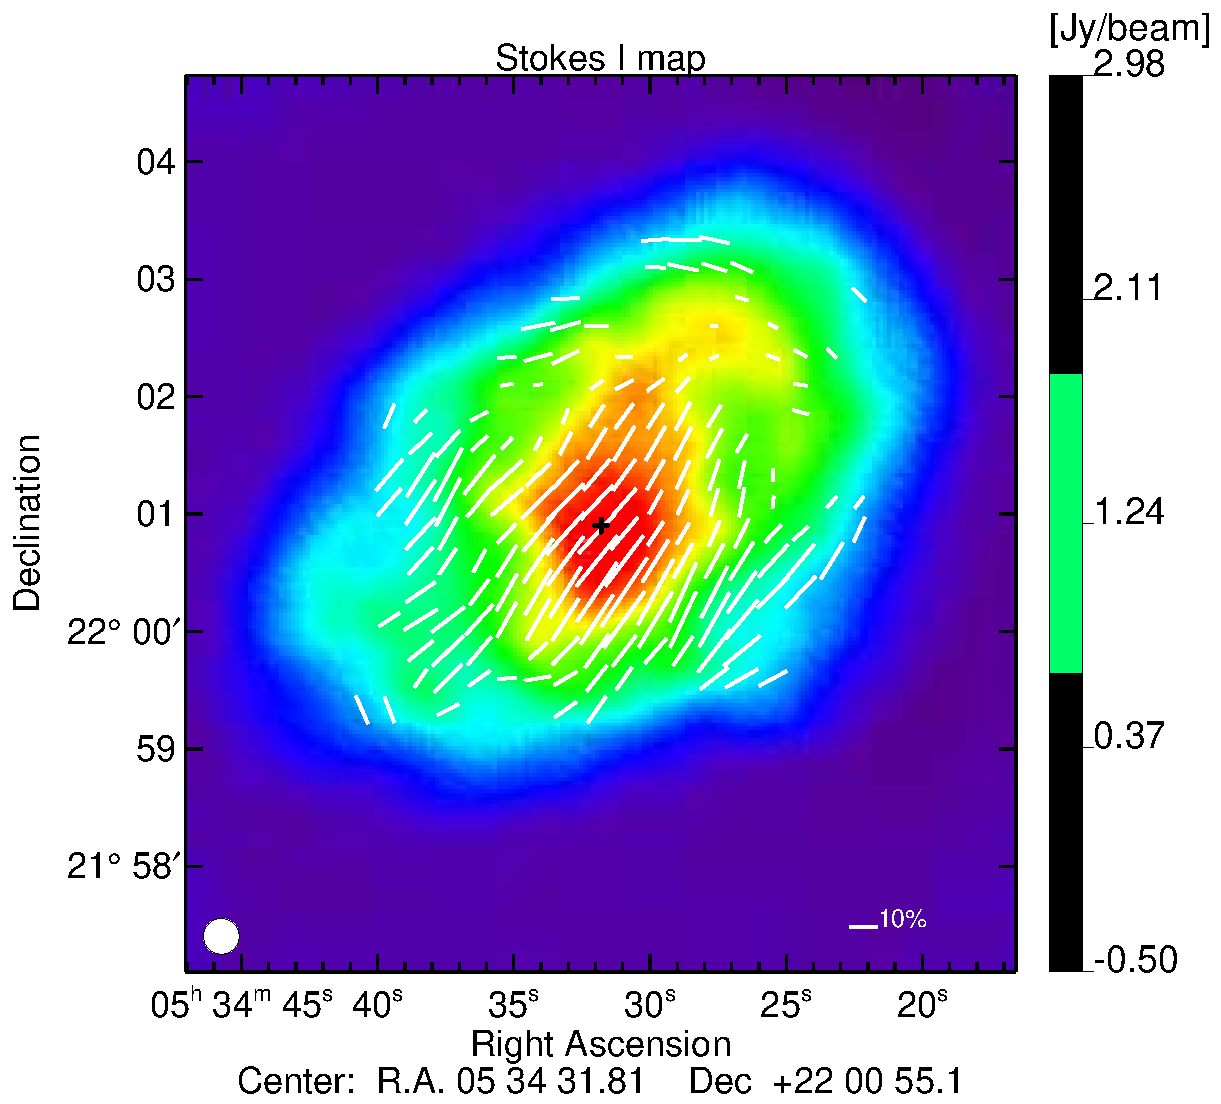
\includegraphics[width=0.32\linewidth,keepaspectratio]{figures/Crab_i_v3.pdf}}	
	     { 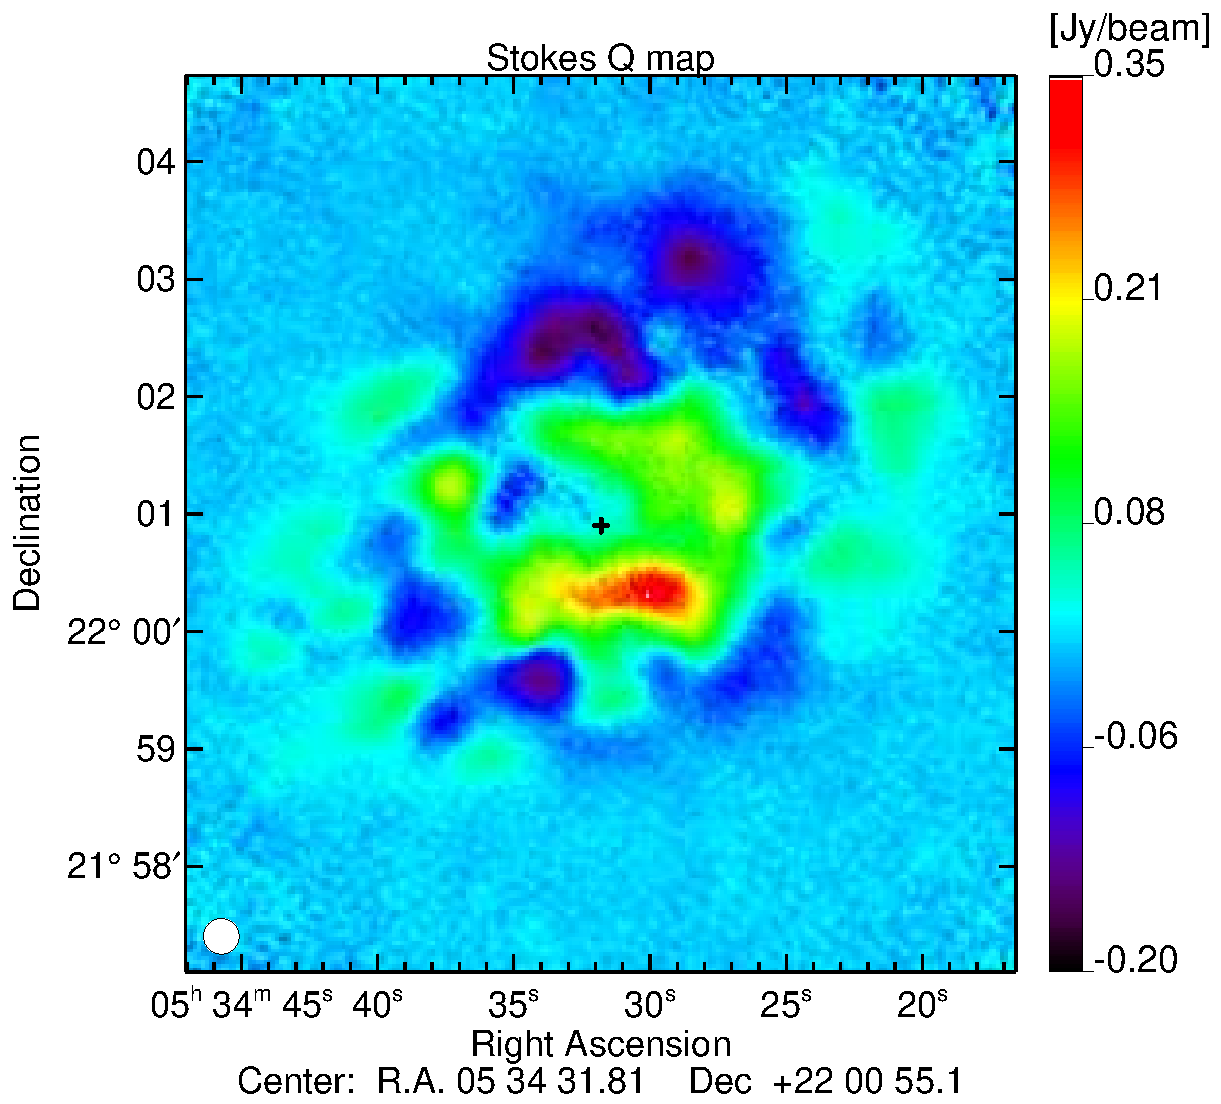
\includegraphics[width=0.32\linewidth,keepaspectratio]{figures/Crab_Q_v3_2mm.pdf}}
          { 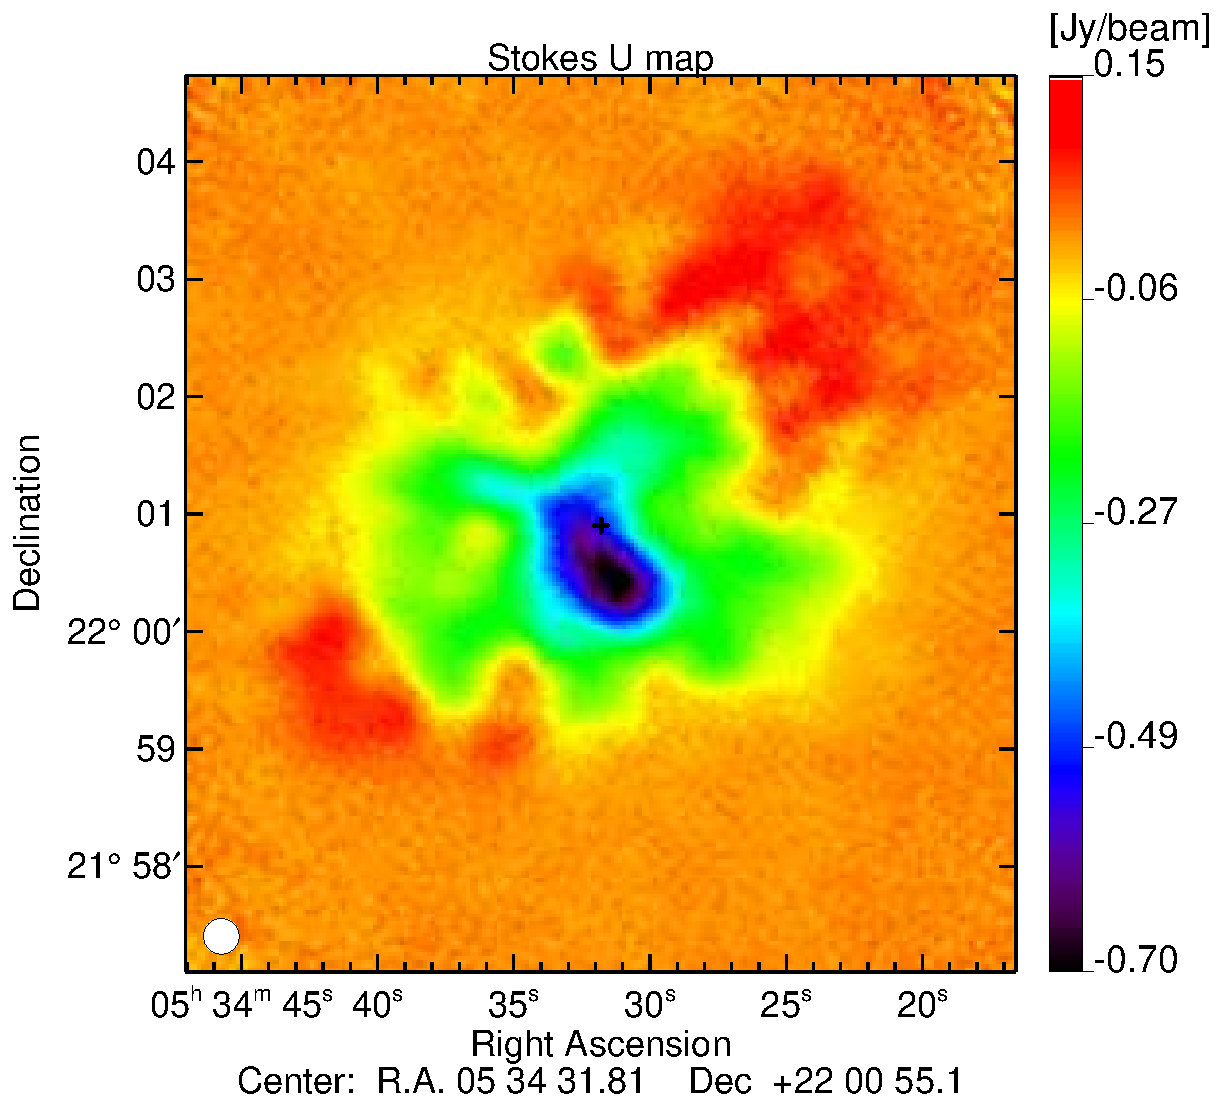
\includegraphics[width=0.32\linewidth,keepaspectratio]{figures/Crab_U_v3_2mm.pdf}} 
           \caption{From left to right: Crab nebula Stokes $I$, $Q$ and, $U$
             maps shown here in Equatorial coordinates obtained at 150 GHz with the \NIKA\ camera. Polarization
             vectors, indicating both the polarization degree and the orientation, are
             over-plotted in blue on the intensity map where the polarization
             intensity satisfies $I_{pol} > 3 \sigma_{I_{pol}}$ and $I_{pol} >$ 0.1 Jy/beam. In each map, the \NIKA\ FWHM is shown as a white disk in the bottom left-hand corner and the cross marks the pulsar position.}
\label{crab_intensity_maps}
\end{figure*}


\section{Introduction}\label{sec:introduction}
The Crab nebula (or Tau A) is a plerion-type supernova remnant emitting a highly
polarized signal \citep{1978A&A....70..419W,1991ApJ...368..463M}.
Referring to \citet{2008ARA&A..46..127H}, from inside out the Crab consists of a pulsar, the synchrotron nebula, a bright expanding shell of thermal gas, and a larger very faint freely expanding supernova remnant.

Near the center of the nebula a shock is observed as formed by the jet thermalized and pulsar's ultra-relativistic wind which is confined by the thermal ejecta from the explosion \citep{2000ApJ...536L..81W,2011A&A...528A..11W}.  
The synchrotron emission from the nebula is observed in the radio frequency domain as powered by the pulsar located at equatorial coordinates (J2000) $R.A. = 5^h34^m31.9383014s$ and $Dec. = 22^{\circ}0^{\prime}52.17577^{\prime\prime}$ \citep{Lobanov} through its jet.

The polarization of the Crab nebula radio emission, discovered in 1957 independently by \citet{1957ApJ...126..468M} and \citet{1959SvA.....3...39K}, has confirmed the synchrotron emission is the underlying mechanism. 

Today the Crab nebula is perhaps the most observed object in the sky beyond our own solar system \citep{2008ARA&A..46..127H} and often used as calibrator by new instruments. It is also quite isolated
with low background diffuse emission. 

In particular it is the most intense polarized astrophysical object in the microwave sky
at angular scales of few arcminutes and for this reason it is chosen not only for high resolution cameras
but also for the calibration of
CMB (Cosmic Microwave Background) polarization experiments, which have
beamwidths comparable to the extension of the source. 
%The polarization of the Cosmic Microwave Background (CMB) anisotropies offers a
%powerful way to investigate the early Universe. It can be decomposed into a
%scalar and a pseudo-scalar field, respectively called $E$ and $B$ modes. The
%primordial density fluctuations (scalar perturbations) can only produce $E$ type
%CMB polarization, while $B$ type CMB polarization can only be produced by
%primordial (tensor perturbations) gravitational waves
%\citep{polnarev1985polarization, 1997PhRvL..78.2054S} arising from the
%inflationary epoch \citep{PhysRevD.23.347, linde1982new} and by gravitational
%lensing of the $E-$modes (\cite{ade2015planck} and refs. therein).  
%The detection of the primordial $B-$modes would set tight constraints on
%Inflation models and constitutes one of the most ambitious goals of modern
%observational cosmology.
%Recently, \citet{bicepplanck2015,bicep2016} set a 95\% upper limit for the
%detection of the tensor to scalar ratio $r$ $\textless$ 0.07.  
Indeed, upcoming CMB experiments aiming at measuring the primordial $B-$modes require an accurate
determination of the foreground emissions to the CMB signal and a high control
of systematic effects.
% One of the most difficult parameters to be characterized
%for a CMB polarization experiment is the calibration of residual cross
%polarization and of the absolute polarization angle. This can be achieved using
%observations of well known polarized sources like the Crab nebula. 
The Crab nebula has already been used for polarization cross-check analysis in the frequency
range from 30 to 353 GHz \citep{2011ApJS..192...19W,2015arXiv150702058P}.

High angular resolution observations from the XPOL experiment \citep{thum2008} at the
IRAM 30 m telescope have revealed the spatial distribution of the Crab Nebula in
intensity and polarization at 90 GHz with an absolute accuracy of 0.5$^{\circ}$
in the polarization angle \citep{aumont2010}.
This observation has also shown that the polarization spatial distribution varies from the source peak
to the edges of the source and evidences the need of an accurate study at high resolution in a large frequency range to be able to use this source as a calibrator for future polarization esperiments.

%, in particular those aiming at a precise measurement
%of the CMB polarization that have a large frequency range to be able to
%carefully study and subtract foreground emission \citep{2016IJMPD..2540008K}.

Previous studies \citep{macias2010} of the total Spectral Energy Distribution
(SED) have shown a spectrum well described by a single
synchrotron component at radio and mm wavelengths and predict negligible
variations in polarization fraction and angle in the frequency range of interest
for CMB studies.
 
Observations of the Crab nebula polarization have been performed with the
\NIKA\ camera \citep{monfardini2010,catalano2014,monfardini2014} at the IRAM 30
m telescope during the observational campaign of February, 2015. A first
overview of the \NIKA/30m Crab polarization observations,
focusing on instrumental characterization of the polarization system, was given in
\cite{2016JLTP..184..724R}. In this paper we go a step further in the analysis
by combining \NIKA/30m (\NIKA\ from here on) observations with published values at other frequencies, and spanning different angular resolutions, to trace the
SED in total intensity and polarization of the Crab nebula. As far for polarization we use observations from the \WMAP\
satellite at 23, 33, 41, 61 and 94 GHz \citep{2011ApJS..192...19W}, from the
\Planck\ satellite at 30, 44, 70, 100, 143, 217, 353 GHz and from XPOL/30m (XPOL from here on) at 90 GHz
\citep{aumont2010} and POLKA/APEX (POLKA from here on) at 345 GHz \citep{2014PASP..126.1027W}. 


The paper is organized as follows: in Sec.~\ref{sec:NIKA observations} the
intensity and polarization maps obtained with the \NIKA\ camera are presented
together with the polarization degree and angle spatial distributions;
Sec.~\ref{sec:Polarization estimates in CMB experiments like beams} presents the
reconstruction of the polarization properties of the Crab nebula in well defined
regions; Sec.~\ref{sec:Polarization intensity Spectral Energy Density (SED)}
presents the Crab nebula SED in total intenstity and polarization; in
Sec.~\ref{sec:conclusions} we present our conclusions.
 
\section{\NIKA\ observations of the Crab Nebula}\label{sec:NIKA observations}
\subsection{\NIKA\ camera and polarization setup}\label{sec:nika camera}
\NIKA\ is a dual band camera observing the sky in intensity and polarization at
150 and 260 GHz with 18~arcsec and 12~arcsec FWHM resolution, respectively. It
has a Field-of-View (FoV) of 1.8$^{\prime}$ at both wavelengths. It was operated at the
IRAM 30~m telescope between 2012 and 2015. A detailed description of the
\NIKA\ camera can be found in \citet{monfardini2010, monfardini2011} and
\citet{catalano2014}.

In addition to total power observations, \NIKA\ was also a test
bench for the polarization system of the final instrument
\NIKAd\ \citep{calvo2016,catalano2016nika2,2017arXiv170700908A}, which was installed at the
telescope in October, 2015. The polarization setup of \NIKA\
consists in a continuously rotating metal mesh half wave plate (HWP)
followed by an analyzer, both at room temperature and placed in
front of the entrance window of the cryostat. The \NIKA\ Lumped Elements Kinetic
Inductance Detectors (LEKIDs) are not intrinsically sensitive to
polarization. The HWP rotates at 2.98 Hz allowing a modulation of the polarization signal at $4\times 2.98$~Hz while the typical telescope scanning speed is equal to 26.23 arcsec/s.
The conditions provide a quasi-simultaneous measure of Stokes parameters $I$, $Q$ and $U$
per beam and place the polarized power in the frequency domain far from the low frequency
electronic noise and the atmospheric fluctuations. \cite{ritacco2017} give more
details on the \NIKA\ polarization capabilities and describes the performance of
the instrument at the telescope. In particular the sensitivity of the
\NIKA\ camera in polarization mode was estimated to be 50 mJy.$s^{1/2}$ at 150
GHz.

\NIKA\ has provided the first polarization
observations performed with Kinetic Inductance Detectors, confirming that KIDs are a
suitable detector technology for the development also of the next generation of polarization sensitive
experiments.

\subsection{\NIKA\ observations}\label{sec:nika_observations}
Observations of the polarized emission from the Crab nebula with the \NIKA\ camera were performed at
the IRAM 30~m telescope in February, 2015. The average opacity at 150 GHz was $\tau$ = 0.2.  Fig.~\ref{crab_intensity_maps} shows
the Stokes $I$, $Q$ and $U$ maps obtained by a co-addition of 14 maps
of $8 \times 6$ arcminutes for a total observation time of $\sim$ 2.4 hours. The rms calculated on jack-knife noise maps is 36 mJy/beam on Stokes $I$ and 31 mJy/beam on polarization maps Stokes $Q$ and $U$.
The maps were performed in equatorial coordinates in four different scan
directions: 0$^{\circ}$, 90$^{\circ}$, 120$^{\circ}$, 150$^{\circ}$. This
allowed us to have the best mapping with different position angles.

To obtain the Stokes $I$, $Q$, and $U$ Crab nebula maps in Equatorial coordinates, we have used a dedicated
polarization data reduction pipeline \citep{ritacco2017}, which is an extension
of the total intensity \NIKA\ pipeline \citep{catalano2014,adam2013}. The main steps
of the polarization pipeline are summarized below.
\begin{enumerate}
\item Subtraction of the HWP induced parasitic signal, which is modulated at harmonics of the HWP rotation frequency and represents the most tedious noise contributing to the polarized signal. 
\item Reconstruction of the Stokes $I$, $Q$ and $U$ time ordered information
  (TOI) from the raw modulated data. This is achieved using a demodulation
  procedure consisting in a lock-in around the fourth harmonic of the HWP rotation frequency, where the polarization signal is located.
\item Subtraction of the atmospheric emission in the demodulated TOIs using
  decorrelation algorithms. In polarization, the HWP modulation reduces
  significantly the atmospheric contamination and there is no need to
  further decorrelate the $Q$ and $U$ TOI's from residual atmosphere. By contrast, in
  intensity the atmospheric emission fully dominates the signal and, to recover
  the large angular scales, we use the 260~GHz band as an atmosphere
  dominated band like in \cite{adam2013}.  This decorrelation impacts the
  reconstructed Stokes maps via a transfer function. We have estimated this function
  with simulated observations of diffuse emission that were passed through the
  data reduction pipeline, with the exact same scanning, sample flagging and data
  processing as real data. We found that the power spectrum of the output maps
  match that of the input one to better than 1\% (~5\%) on scales smaller
  (resp.~larger) than $\sim 1'$, see Fig.~\ref{transfer_func}. The impact of the data processing is thus
  negligible compared to uncertainties on absolute calibration on small
  scales, and its moderate effect on large angular scales is further reduced
  with the subtraction of a zero level for the photometry (see below). In the
  following, we therefore neglect the impact of this transfer function.


\item Correction of the intensity-to-polarization-leakage-effect, which was
  identified in observations of unpolarized sources like the planet Uranus. For
  point sources the effect was about 3\% peak-to-peak, while for extended sources like the Crab nebula it has been found to be the order of 0.5 \% peak-to-peak. 
  \cite{ritacco2017} describe the algorithm of leakage correction developed specifically for \NIKA\ polarization observations. Applying this algorithm to Uranus observations the instrumental polarization is reduced to 0.6\% of the total intensity $I$.
  \item Projection of the demodulated and decorrelated Stokes $I$, $Q$, and $U$ TOIs into Stokes $I$, $Q$ and $U$ equatorial coordinates maps.

\end{enumerate}

\begin{figure}[h!]
  \centering
  \includegraphics[width=0.7\linewidth,keepaspectratio]{figures/Crab_transfer_func.eps}
	\caption{Transfer function of the data processing in total intensity.}
\label{transfer_func}
\end{figure}
  
  \begin{figure*}
\centering
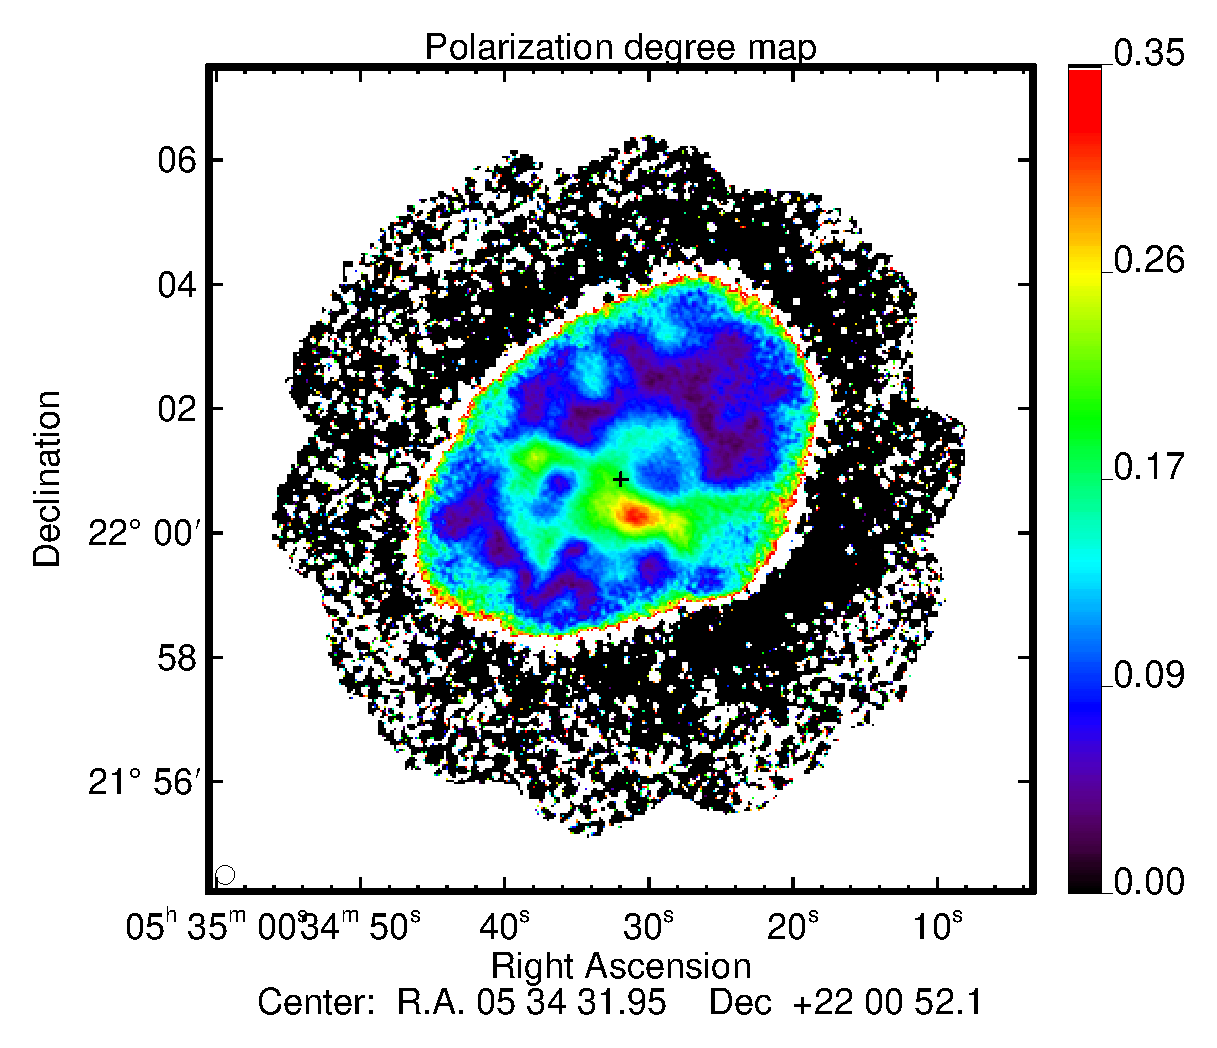
\includegraphics[clip, angle=0, scale = 0.35]{figures/Crab_pol_deg_v3.pdf}
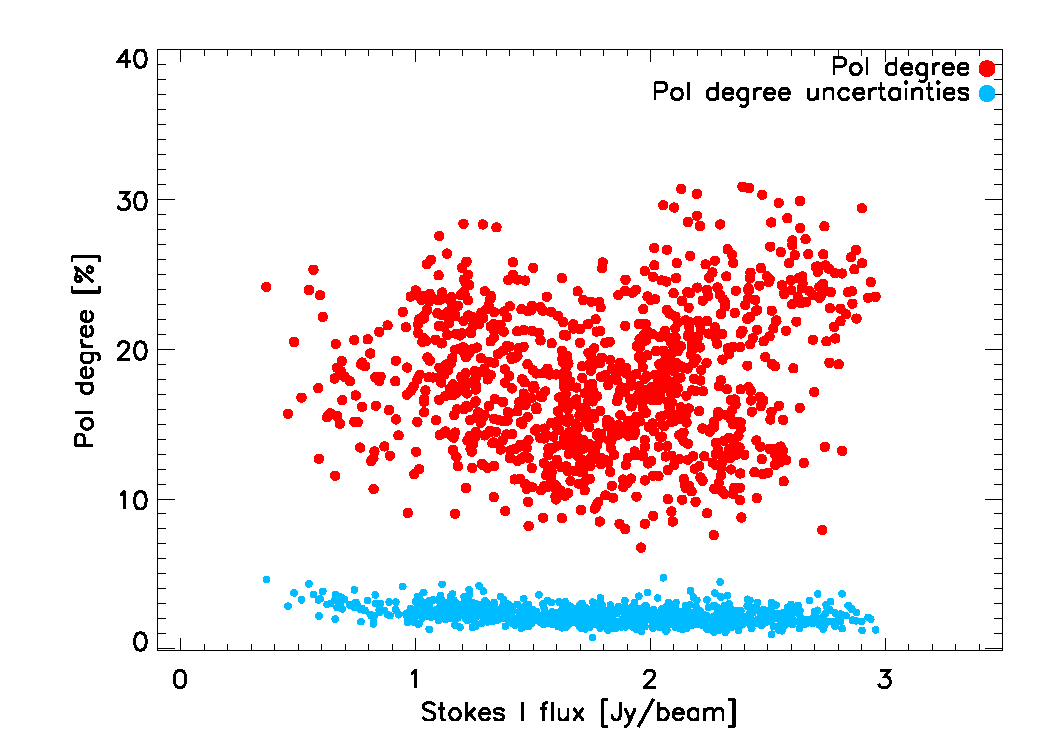
\includegraphics[clip, angle=0, scale = 0.5]{figures/pol_deg_vs_I_2mm.pdf}
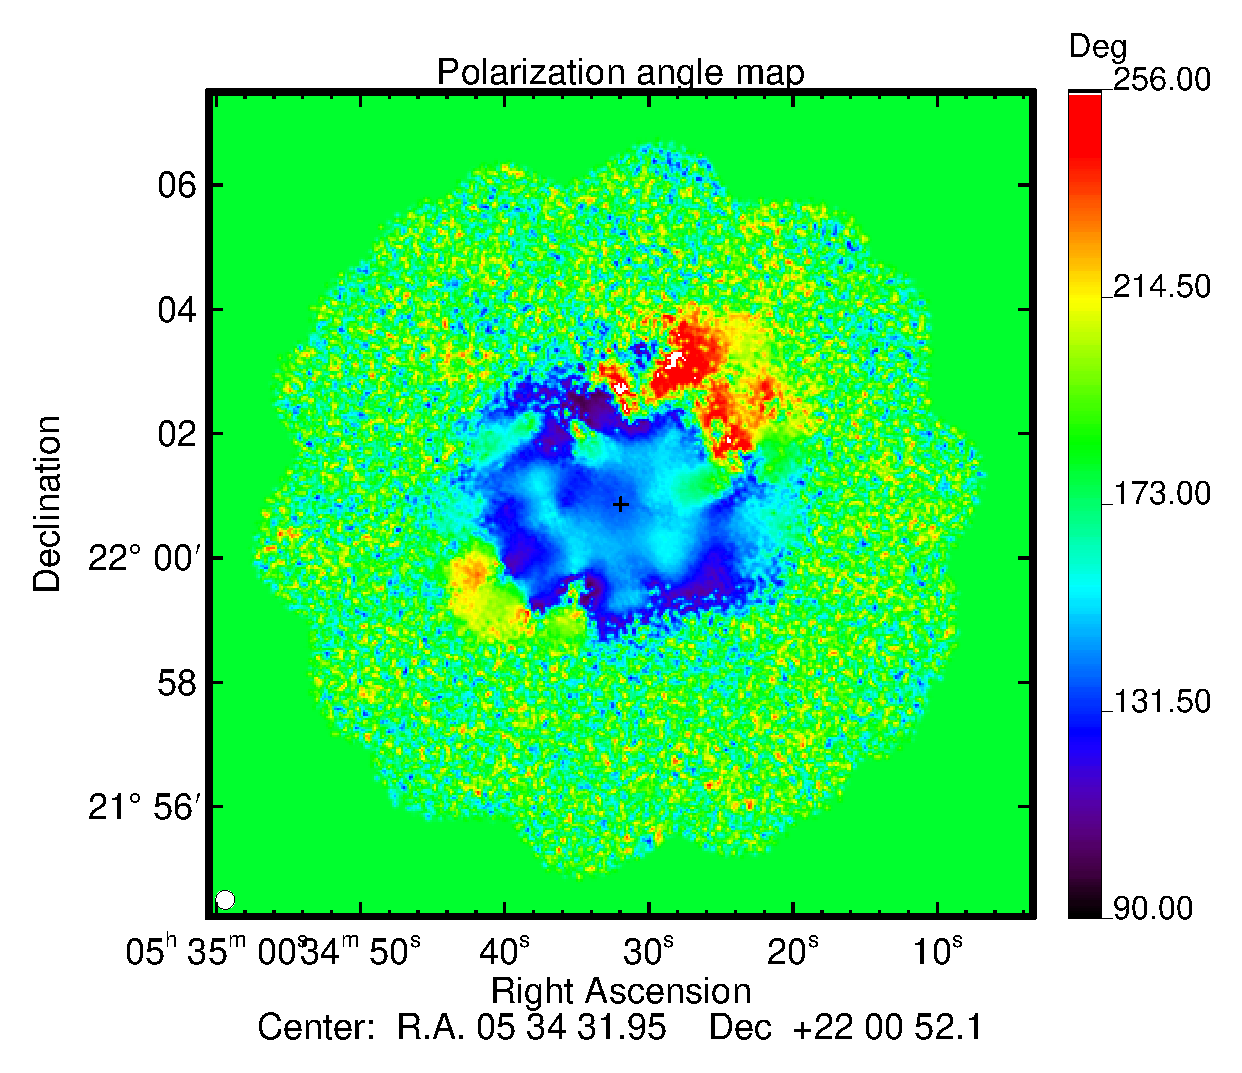
\includegraphics[clip, angle=0, scale = 0.35]{figures/Crab_angle_v3_2mm.pdf}
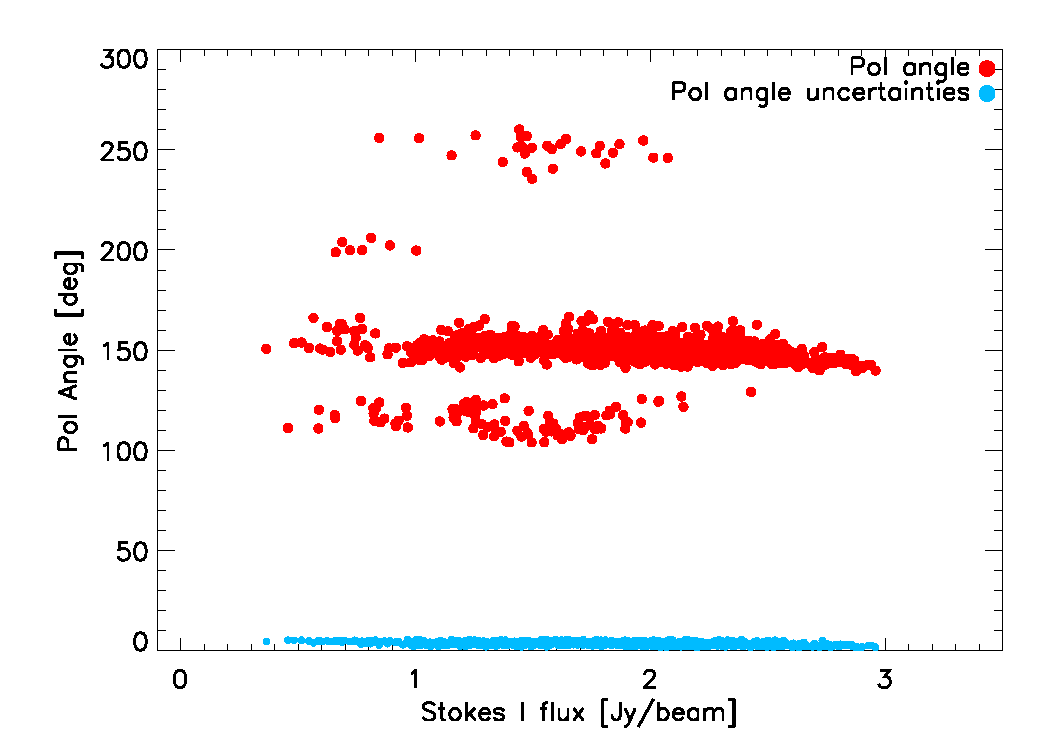
\includegraphics[clip, angle=0, scale = 0.5]{figures/pol_angle_vs_I_2mm.pdf}
\caption{{\it Top}: The left panel shows the polarization
  degree map $p$, uncorrected for noise bias, of the Crab nebula. The right panel shows the noise bias
  corrected $p$ values as a function of total intensity map (Stokes $I$). The
  condition $I_{pol}$ $\textgreater$ 5$\sigma_{I_{pol}}$ is satisfied for those values. {\it
    Bottom}: on the left we present the polarization angle map $\psi$ (Equatorial coordinates system) of the
  Crab nebula. On the right panel the distribution of $\psi$ values is
  represented as a function of the total intensity in the case of very high S/N ratio where $I_{pol}$ $\textgreater$ 5$\sigma_{I_{pol}}$ . The cyan dots represent the uncertainties calculated as the
  dispersion between different observational scans. The black cross marks the pulsar position on the maps.}
\label{fig:pol_degree}
\end{figure*}
 \begin{figure}
  \centering
      {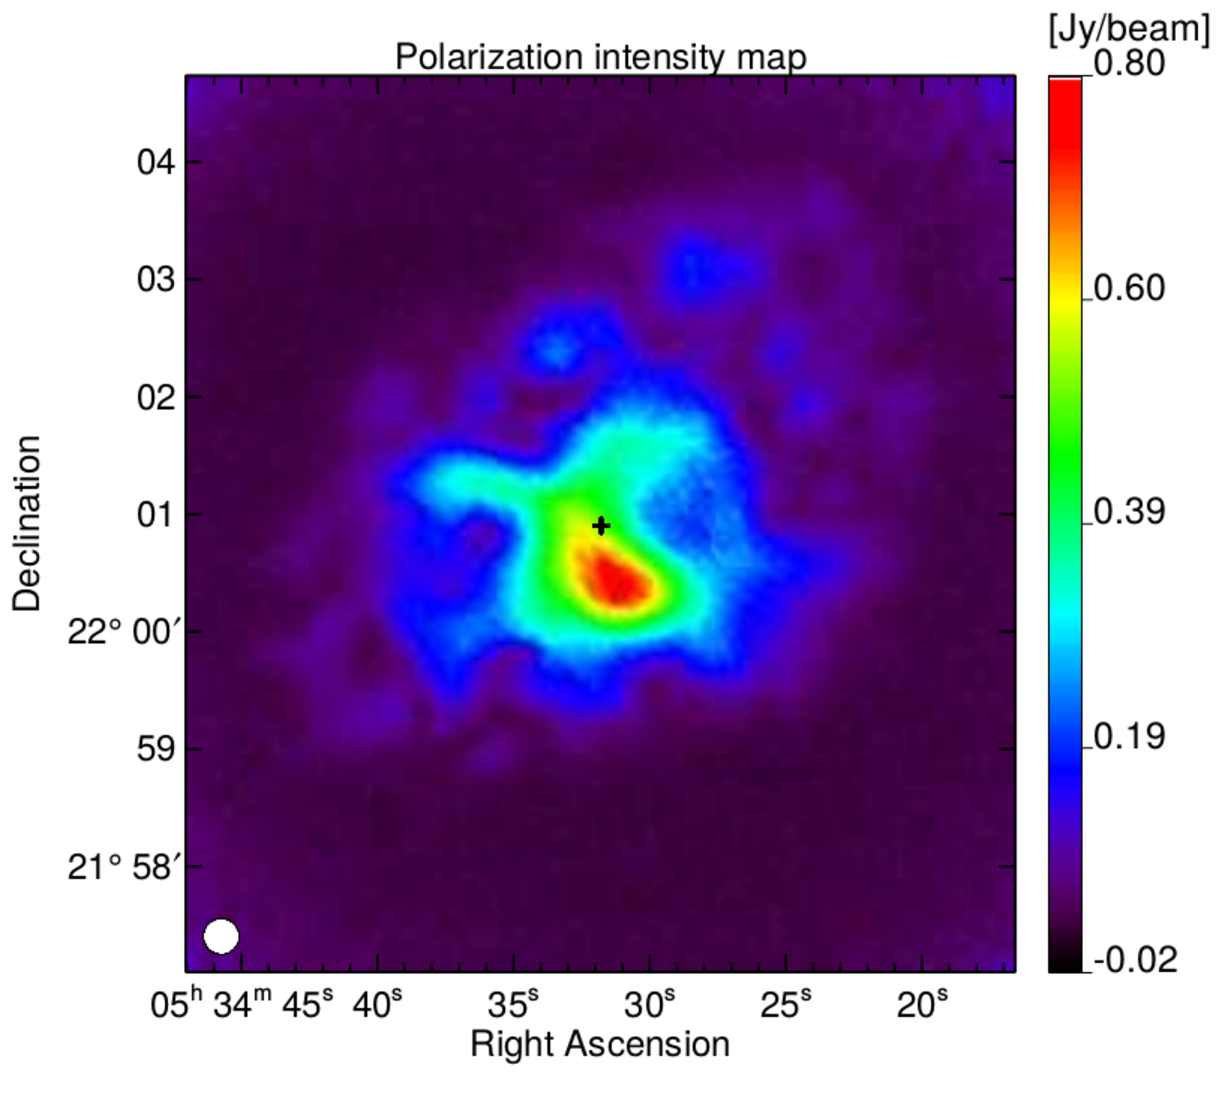
\includegraphics[width=0.75\linewidth,keepaspectratio]{figures/Crab_ipol_v3_2mm.pdf}}
\caption{\NIKA\ polarized intensity map of the  Crab nebula at 150 GHz. The map shows high polarized emission reaching a value of 0.8 Jy beam$^{-1}$. The telescope beam FWHM is shown in the lower left. The black cross marks the pulsar position.}
\label{crab_ipol_maps}		
  \end{figure}
 


\subsection{Crab polarization properties}\label{sec:pol_properties}
In this section we discuss the polarization properties of the source in terms of polarization degree $p$ and angle $\psi$, which are defined through the Stokes parameters $I, Q$, and $U$ as follows:
\begin{equation}
 p    = \frac{\sqrt{Q^2 + U^2}}{I} \nonumber 
\end{equation}
and
 \begin{equation}
 \psi = \frac{1}{2}\arctan\frac{U}{Q}.\label{angledegree_polar}
 \end{equation}
The polarization angle follows the IAU convention, which counts East from North in the equatorial coordinate system.

These definitions are not linear in $I$, $Q$ and $U$ and therefore, the observational uncertainties have to be carefully considered, {\it i.e.} $p$ and $\psi$ are noise biased. 
\citet{1980A&A....91...97S,1985A&A...142..100S,montier} proposed analytical solutions to correct for this bias. For intermediate and high S/N ratio the polarization degree and its uncertainty read:
 \begin{eqnarray}
 p    &=& \frac{\sqrt{Q^2 + U^2 - \sigma_{Q}^2 - \sigma_{U}^2}}{I}, \nonumber \\ 
  \sigma_{p} &=& \frac{\sqrt{Q^2\sigma_Q^2 + U^2\sigma_U^2 + p^4I^2\sigma_I^2}}{pI^2}.
  \label{p_true_degree}
 \end{eqnarray}
 Furthermore, the polarization angle in a high S/N regime can be approximated by Eq.~\ref{angledegree_polar} with the uncertainty
  \begin{eqnarray}\label{angle_uncertainty}
  \sigma_{\psi} = \frac{\sqrt{Q^2\sigma_Q^2 + U^2\sigma_U^2}}{2(pI)^2}.
  \end{eqnarray}

The spatial distribution map of the polarization degree $p$ of the Crab nebula
without noise bias correction is presented on the top left panel of
Fig.~\ref{fig:pol_degree}. Notice that we have set to 0 the pixels for wich the total intensity is lower than 0.1 Jy/beam to avoid the divergence of $p$. Same has been done for the polarization angle map (bottom left of Fig.~\ref{fig:pol_degree}.)

The polarization degree $p$ reaches a value of 20.9 $\pm$0.8 \% at
the peak of the total intensity, which is consistent with what is observed on the
top right panel of Fig.~\ref{fig:pol_degree}, where the variation of $p$ as a
function of the Stokes $I$ is shown.  Here the $p$ values have been noise bias
corrected and satisfy the condition $I_{pol}=\sqrt{Q^2+U^2}$ $\textgreater$ 5
$\sigma_{I_{pol}}$. The distribution of the polarization degree appears highly
dispersed around a mean value of 20\%.  The compatibility between the $p$ value
computed at the Stokes $I$ peak position and the above mentioned plot is
expected because we use a very high S/N ratio threshold of 5 $\sigma_{I_{pol}}$,
which restricts the measurement to a small region around the peak of the source.
%In addition, the $p$ value found is also consistent within the error bars with
%POLKA/APEX experiment measurement \citep{2014PASP..126.1027W} (cf.~Table~\ref{tab:peak_pulsar_others}).
                                 %The polarization degree decreases towards the edges of the source. Furthermore, the high polarization degree observed at the extremities of the source is misleading and caused by the very low S/N ratio of the Stokes $I$ map observed in these regions.
The spatial variation of $p$ highlights the interest of high resolution polarization
observations of the Crab nebula. 

The bottom left panel of Fig.~\ref{fig:pol_degree} shows the spatial distribution of polarization angle
$\psi$. As discussed in \cite{ritacco2017} a 1.8$^{\circ}$ uncertainty must be considered in the polarization angle coming from the determination of the HWP zero position, corresponding to its optical axis in the \NIKA\ cabin reference frame. An uncertainty of 0.5$^{\circ}$ must be considered due to the leakage effect subtraction, which has been estimated from the comparison of the maps before and after leakage correction. We observe a relatively constant polarization
angle 140$^{\circ}$ $\textless$ $\psi$ $\textless$150$^{\circ}$ represented here in equatorial coordinates, except
for the northern-east region where the averaged angle is around $250^{\circ}$, and
some inner regions with lower polarization angle.  These values are confirmed by
the bottom right panel that shows the polarization angle distribution as a
function of total intensity satisfying the condition $I_{pol} > 5\sigma_{I_{pol}}$.

The sudden change of polarization angle on the northern region was already
observed by the XPOL experiment at 90 GHz \citep{aumont2010}.  This together
with the variation of the polarization fraction discussed above confirms the
need of high angular resolution observations at low and high frequencies for a
good understanding of the Crab polarized emission properties.
High resolution observations give the possibility to estimate the polarization properties at different scales and compare with low resolution experiments, like CMB experiments.

We present in Fig.~\ref{crab_ipol_maps} the 150 GHz Crab polarization intensity
map $I_{pol}$ uncorrected for noise bias. We observe a peak at 0.8 Jy beam$^{-1}$ and the polarization
decreases towards the edges of the nebula.

\subsection{Comparison to other high resolution experiments}
Following previous studies, we compare here \NIKA\ results at the pulsar position and at Stokes $I$ map peak with high angular resolution experiments such as POLKA, XPOL and SCUPOL/JCMT (SCUPOL from here on). These experiments observed at wavelengths of 870 $\mu$m, 3 mm and 850 $\mu$m, respectively.
Tab.~\ref{tab:peak_pulsar_others} reports the measurement of the polarization properties, degree and angle, obtained by these experiments \citep{2014PASP..126.1027W}. 
At the pulsar position we observe fair agreement in the polarization angle between POLKA, SCUPOL and \NIKA. However, in terms of polarization degree there is not clear consistency. At the position of the peak in total intensity, \NIKA\ shows a low polarization degree, but still consistent with SCUPOL. Some of the discrepancies observed in Tab.~\ref{tab:peak_pulsar_others} may come from the different pixel resolution of the maps. Indeed being the pizel size different for each map, the computation of the values at the Stokes $I$ peak or at the pulsar position is misleading.

\begin{table}[h!]
  \centering
      \begin{tabular}{ccccccccc}
      \hline
      \hline
      & &  \small Pulsar & & \\
       & \small $I$ [Jy]& \small $p$ [\%] & \small $\psi$ [$^\circ$] & \\ 
       \hline
      \small POLKA   & \small 1.63 & \small 25.3 $\pm$ \small 3.0 & \small 145.1 $\pm$ \small 3.3 & \\
      \small XPOL     & & \small 13.9 $\pm$ \small 0.6 & \small 158.1 $\pm$ \small 0.5 &  \\
      \small SCUPOL &  & \small 14.3 $\pm$ \small 1.8 & \small 140.0 $\pm$ \small 2.8& \\
      \small \NIKA\ & \small 1.2 $\pm$ \small 0.13 & \small 17.5 $\pm$ \small 0.7 & \small 137.8 $\pm$ \small 0.5 $\pm$ \small 0.5 $\pm$ \small 1.8\\
      \hline
      \hline
       & &  \small Peak & & \\
       \hline
      \small POLKA & \small 1.72 & \small 25.0 $\pm$ \small 3.1 & \small 151.7 $\pm$ \small 3.5 &  \\
      \small XPOL  & &  \small 21 $\pm$ 1.2 & \small 149.0 $\pm $ \small 1.4 &  \\
      \small SCUPOL &  & \small 18.7 $\pm$ 1.5 & \small 146.1 $\pm$ \small 2.1&\\
  \small \NIKA\ &  \small 1.22 $\pm$ \small 0.12 & \small 19.8 $\pm$ \small 0.7 & \small 140.0 $\pm$ \small 0.1 $\pm$ \small 0.5 $\pm$ \small 1.8\\
     \hline            
    \hline   
    \end{tabular}
   \caption{ Values estimated by POLKA (870 $\mu$m), XPOL (3 mm), SCUPOL (850 $\mu$m) reported in \cite{2014PASP..126.1027W} and \NIKA\ (this paper) at the pulsar and peak position, respectively. The FWHM for these four experiments are 20$^{\prime\prime}$, 27$^{\prime\prime}$, 20$^{\prime\prime}$ and 18.2$^{\prime\prime}$, respectively. For \NIKA\ the position of the pulsar, represented on the maps by a black cross, refers to \cite{Lobanov}. The position of the peak of the total intensity measured on \NIKA\ maps has equatorial coordinates (J2000) $R.A. =5^h34^m32.3804s$ and $Dec. = 22^{\circ}0^{\prime}44.0982^{\prime\prime}$. The polarization angle is given here in Equatorial coordinates. A systematic angle uncertainty of 2.3$^{\circ}$ is considered. A total calibration error of 10 $\%$ has been accounted for and propagated to the polarization estimates.}
\label{tab:peak_pulsar_others}
 \end{table}



\section{Total intensity and polarization fluxes}\label{sec:Polarization estimates in CMB experiments like beams}
We compute the total flux across the Crab nebula, which has an extent of about
5$^{\prime}$x7$^{\prime}$ as shown in Fig.~\ref{crab_intensity_maps}.  We use
standard aperture photometry techniques to calculate the flux as shown on the top panel of
Fig.~\ref{crab_integrated_flux}. We use as center position the center of the
map with equatorial coordinates (J2000) $R.A. = 5^h34^m31.95s$ and $Dec. = 22^{\circ}0^{\prime}52.1^{\prime\prime}$. A zero level in the map, calculated as the mean of the signal measured on
an external annular ring region (see bottom panel of
Fig.~\ref{crab_integrated_flux}) of radius 4$^\prime$ $\textless$ R $\textless$
4.5$^\prime$, has been subtracted from the map. The total signal estimated is
209.9$\pm$1.0$\pm$5.1$\pm$21.0 Jy. The first uncertainty term accounts for statistical
uncertainties computed from fluctuations of the signal at large radii. The second uncertainty accounts for the difference between two sets of jack-knife noise maps. The latter one accounts for the absolute calibration error of 10\%.
We use Uranus for absolute point source flux calibration. The flux of the planet is estimated from a frequency dependent model of the planet brightness temperature as described in \cite{moreno2010}. 
This model is integrated over the \NIKA\ bandpasses for each channel, and it is assumed to be accurate at the 5\% level. The final absolute calibration factor is obtained by fitting the amplitude of a Gaussian function of fixed angular size on the reconstructed maps of Uranus, which represents the main beam. For the polarization observational campaign of February 2015 this uncertainty is estimated to be 5\% for the \NIKA\ 2.05 mm channel (150 GHz) \citep{ritacco2017}. 
Nevertheless, as described in \cite{adam2013, catalano2014}, by integrating the Uranus flux up to 100 arcsec, we observe that the total solid angle covered by the beam is larger than the Gaussian best-fit of the main beam by a factor of 28\%. As a consequence we account for this factor in the estimation of the fluxes.
Moreover, \cite{adam2013} estimated the uncertainty on the solid angle of the main beam to be 4\%.
Finally, the overall calibration error is estimated to be about 10\%, by considering also the uncertainties on the side lobes.

The polarization efficiency factor estimated across the \NIKA\ 2.05 mm spectral band and reported in \cite{ritacco2017} is $\rho_{pol}$ = 0.9941 $\pm$ 0.0002. This very small efficiency loss of 0.6 \% has a negligible impact on the estimation of the polarization fluxes and the calibration error itself. 

\begin{figure}[h!]
  \centering
 % \includegraphics[width=0.7\linewidth,keepaspectratio]{figures/Crab_transfer_func.eps}f
  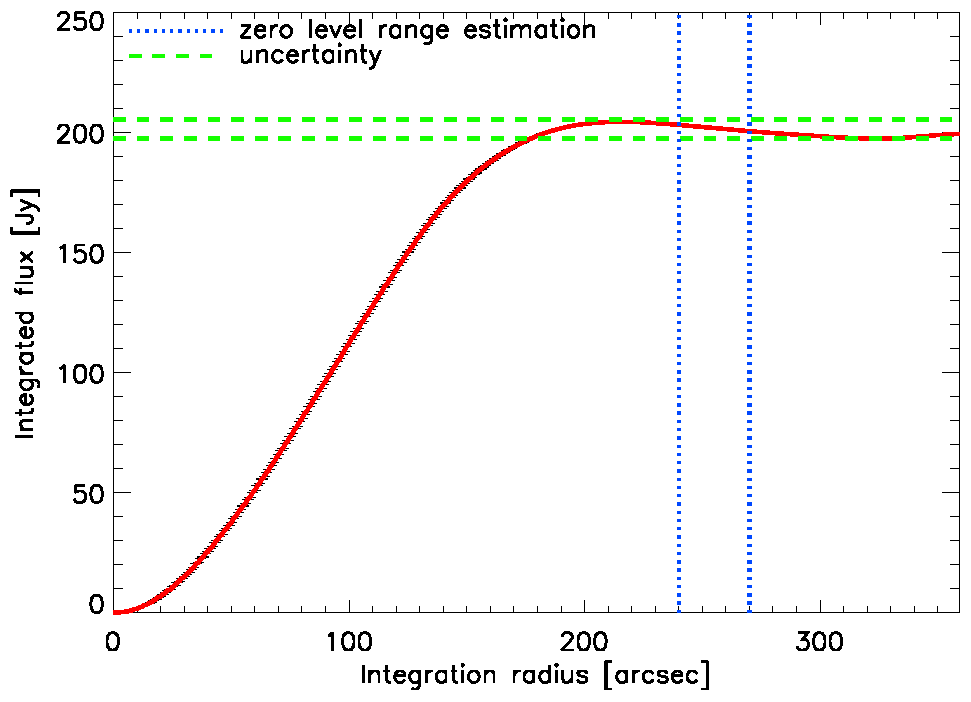
\includegraphics[width=0.7\linewidth,keepaspectratio]{figures/Crab_integrated_flux_2mm.pdf}
  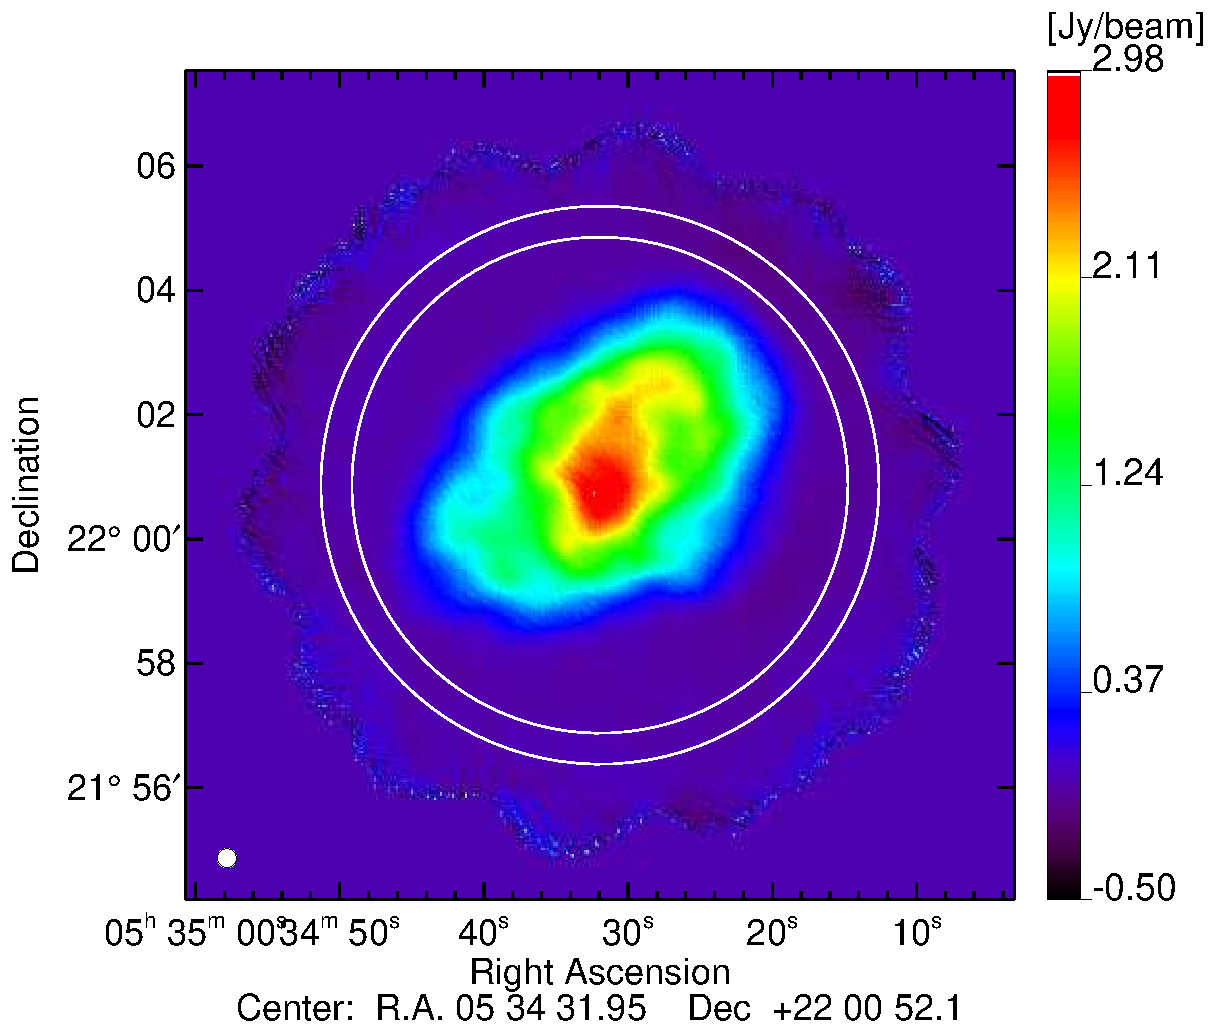
\includegraphics[width=0.8\linewidth,keepaspectratio]{figures/Crab_I_v3_2mm_ring.pdf}
     \caption{
       Cumulative flux of the Crab nebula (top) obtained at 150 GHz over
       4$^{\prime}$ from the center obtained by aperture photometry. The flux
       has been corrected by a zero level in the map, which corresponds to the
       mean of the signal calculated in an annular ring as indicated by the
       white circles on the map and by the blue dotted lines on the
       top. The green dotted line represents the uncertainties measured at large
       radii.}
\label{crab_integrated_flux}
\end{figure}
\begin{figure}
  \centering
          { 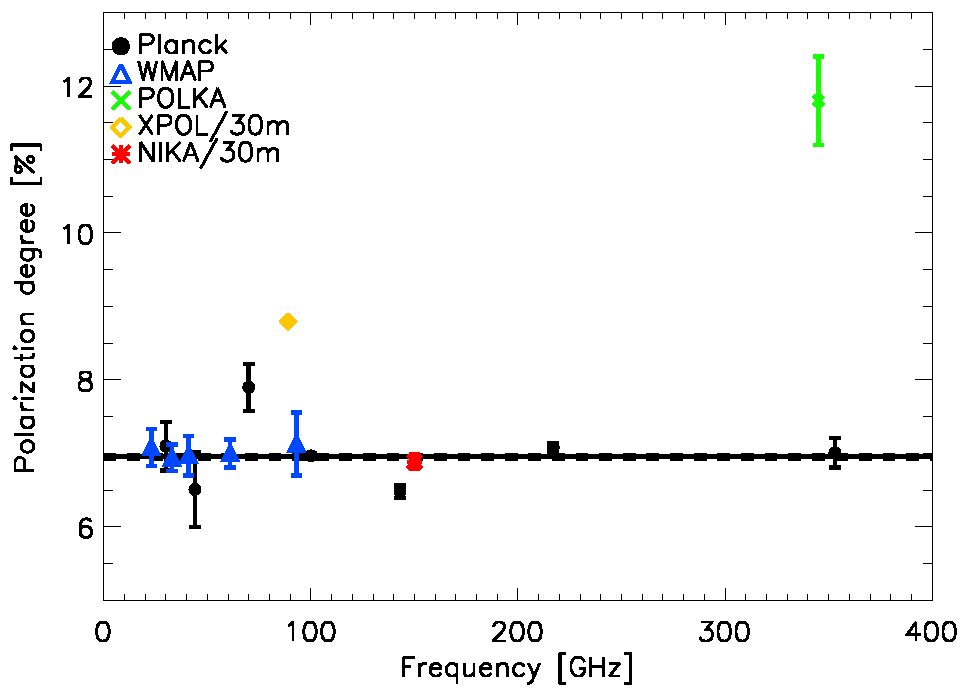
\includegraphics[width=1\linewidth,keepaspectratio]{figures/pdegree_comparison.pdf}}
          { 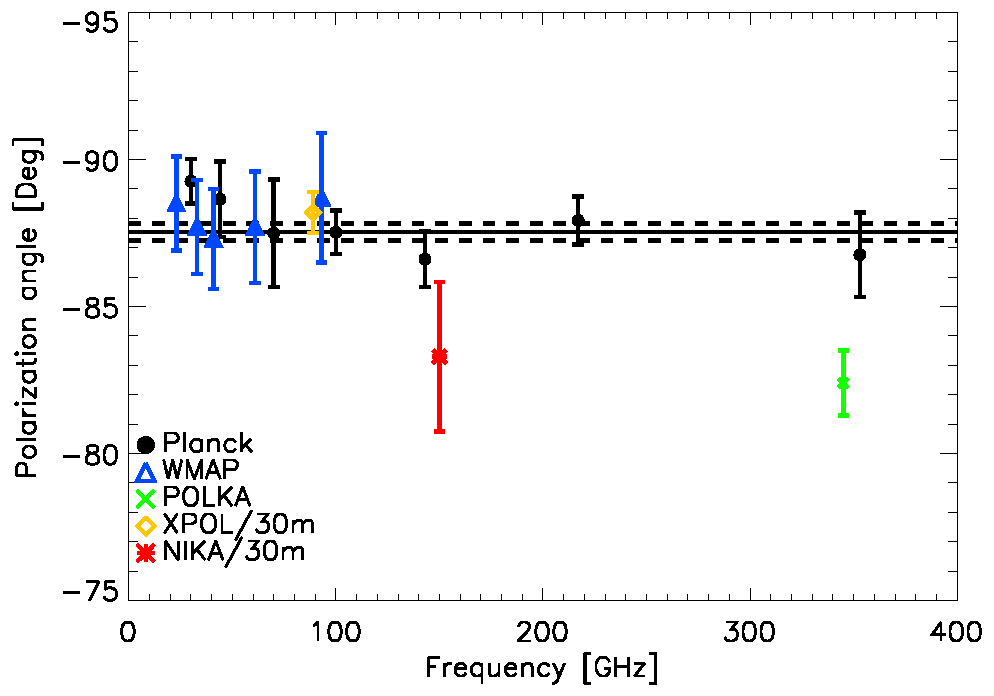
\includegraphics[width=1\linewidth,keepaspectratio]{figures/angle_comparison.pdf}} 
            \caption{{\it Top}: polarization degree as a function of frequency as measured by \Planck\ (black dots), WMAP (blue triangles), XPOL (yellow diamond), POLKA (green cross) and \NIKA\ (red crosses). The \NIKA\ and POLKA values has been estimated by integrating in a radius of $7^{\prime}$. Notice that \Planck\ and WMAP values are shown at their native resolution. XPOL, \NIKA\ and POLKA values have been integrated over the source. The solid line represents the weighted-averaged degree for all experiments but POLKA. Dashed lines represent 1$\sigma$ uncertainties.
            {\it Bottom}: polarization angles in Galactic coordinates for the same five experiments given above. The solid line represents the weighted-averaged polarization angle computed using all the values.}
\label{crab_p_angle_comparison}		
  \end{figure}
\begin{table*}[h!]
  \centering
      \begin{tabular}{ccccccccc}
      \hline
      \hline
       & \small $I$ [Jy] & \small $Q$ [Jy] & \small $U$ [Jy] & \small $I_{pol}$ [Jy] & \small $p$ [\%] & \small $\psi_{eq}$ ($\psi_{gal}$) [$^\circ$] \\
      \hline

%\small 5$^{\prime}$ FWHM centered & \small 198.9$\pm$4.8  & \small 2.8$\pm$0.1 & \small -16.1$\pm$0.2 & \small 16.3$\pm$0.3 & \small 8.2$\pm$0.1 & \small 140.0(-82.4)$\pm$0.2$\pm$0.5$\pm$1.8$^*$ & \small 145.3(-87.6)$\pm$0.1$\pm$0.5$\pm$1.8$^*$ \\ 

%	\small 7$^{\prime}$ FWHM centered & \small 226.4$\pm$5.7 & \small 3.2$\pm$0.2 & \small -15.2$\pm$0.3 & \small 15.6$\pm$0.3 & \small 6.9$\pm$0.1 & \small 140.9(-83.3)$\pm$0.3$\pm$0.5$\pm$1.8$^*$ & \small 145.2(-87.6)$\pm$0.1$\pm$0.5$\pm$1.8$^*$\\ 

\small 5$^{\prime}$ FWHM centered & \small 182.3$\pm$28.5 & \small 2.7$\pm$0.4 & \small -15.3$\pm$1.3 & \small 15.4$\pm$1.6 & \small 8.5$\pm$0.9 & \small 140.0 (-82.4)$\pm$0.2$\pm$0.5$\pm$1.8$^*$  \\ 
\small 7$^{\prime}$ FWHM centered & \small 215.7$\pm$27.9 & \small 3.2$\pm$0.5 & \small -14.1$\pm$1.1 & \small 14.5$\pm$1.4 & \small 6.7$\pm$0.7 & \small 141.4 (-83.8)$\pm$0.5$\pm$0.5$\pm$1.8$^*$ \\ 
\small 10$^{\prime}$ FWHM centered & \small 209.9$\pm$27.1 & \small 3.2$\pm$0.5 & \small -13.2$\pm$0.9 & \small 13.3$\pm$1.3 & \small 6.5$\pm$0.6 & \small 142.0 (-84.3)$\pm$0.6$\pm$0.5$\pm$1.8$^*$ \\ 
\hline            
    \hline   
    \end{tabular}
   \caption{ 
   \NIKA\ Crab nebula total flux $I$, $Q$, and $U$ are here presented, estimated by using aperture photometry methods. Polarized intensity flux $I_{pol}$, polarization degree $p$, and angles $\psi_{eq}$ (Equatorial coordinates) and $\psi_{gal}$ (Galactic coordinates) within parenthesis, are also presented. The values have been calculated within 5$^{\prime}$, 7$^{\prime}$, 10$^{\prime}$, centered on the map center position.
   A total calibration error of 10 $\%$ has been accounted for and propagated to the polarization estimates. The statistical uncertainty accounts also for montecarlo simulation of the noise in $Q$ and $U$ and the differences between two sets of jack-knife maps, 7 each.
 *A systematic angle uncertainty of 1.8$^{\circ}$ must be considered in the polarization angle error budget. We also consider a 0.5$^{\circ}$ of uncertainty due to the intensity to polarization leakage correction.    
    }
    \label{tab:crab_results}
 \end{table*}
 \begin{table*}[h!]
  \centering
      \begin{tabular}{ccccccccc}
      \hline
      \hline
       Frequency [GHz] & \small $I$ [Jy] & \small $Q$ [Jy] & \small $U$ [Jy] & \small $I_{pol}$ [Jy] & \small $p$ [\%] & \small $\psi_{gal}$ [$^\circ$] \\
      \hline

\small 100 & \small 229.23$\pm$0.46  & \small -15.91$\pm$0.07 & \small 1.38$\pm$0.09 & \small 15.97$\pm$0.07 & \small 6.97$\pm$0.03 & \small -87.52$\pm$0.12  \\ 
\small 143 & \small 195.07$\pm$1.24  & \small -12.55$\pm$0.14 & \small 1.49$\pm$0.09 & \small 12.64$\pm$0.14 & \small 6.48$\pm$0.08 & \small -86.61$\pm$0.32  \\
\small 217 & \small 171.36$\pm$0.71  & \small -12.10$\pm$0.08 & \small 0.88$\pm$0.11 & \small 12.14$\pm$0.08 & \small 
7.08$\pm$0.05 & \small -87.93$\pm$0.19  \\
\small 353 & \small 143.20$\pm$0.65  & \small -9.98$\pm$0.29 & \small 1.13$\pm$0.18 & \small 10.05$\pm$0.29 & \small 7.01$\pm$0.20 & \small -86.76$\pm$0.81 \\
    \hline            
    \hline   
    \end{tabular}
   \caption{The same quantities as in Tab.~\ref{tab:crab_results} derived with the new analysis of HFI \Planck\ results by using aperture photometry of the polarization maps published in \cite{refId0}.}
    \label{tab:planck_results}
 \end{table*}



\subsection{Polarization degree and angle estimates}
In order to compare our results with low angular resolution CMB experiments, we present in Tab.~\ref{tab:crab_results} the Stokes $I$, $Q$, and $U$, the polarization intensity, polarization degree $p$ and angle $\psi$. All the listed values are estimated inside apertures with radius of 5$^\prime$, 7$^\prime$ and 10$^\prime$ FWHM from the center of the map.The uncertainties account for the calibration error of 10\%. 
The polarization angle is here presented in Equatorial coordinates and Galactic coordinates to ease the comparison with CMB experiments.
The polarization angle uncertainty accounts for 2.3$^{\circ}$ systematic uncertainties, while the statistical uncertainties for montecarlo simulation of the noise in $Q$ and $U$ and the difference between two sets of jack-knife noise maps, 7 maps each.

% \textbf{
Fig.~\ref{crab_p_angle_comparison} shows the polarization fraction (top) and polarization angle (bottom) of the Crab nebula as a function of the frequency as measured by
five different instruments: 
\WMAP\ \citep{2011ApJS..192...19W}, XPOL \citep{aumont2010}, POLKA \citep{2014PASP..126.1027W}, \Planck\ \citep{2015arXiv150702058P}, and \NIKA\ (this paper). 
Notice that \WMAP\ satellite has FWHMs: 0.93$^{\circ}$, 0.68$^{\circ}$, 0.53$^{\circ}$, 0.35$^{\circ}$, and \textless 0.23$^{\circ}$ at 22 GHz, 30 GHz, 40 GHz, 60 GHz, and 90 GHz respectively. XPOL and POLKA have FWHMs of 27$^{\prime\prime}$ and 20$^{\prime\prime}$, respectively.
The \Planck\ satellite FWHMs are: 33$^{\prime}$, 24$^{\prime}$, 14$^{\prime}$, 10$^{\prime}$, 7.1$^{\prime}$, 5.5$^{\prime}$, and 5$^{\prime}$ arcminutes at 30, 44, 70, 100, 143, 217, and 353 GHz, respectively. Furthermore, after discussions with the \Planck\ team we have reanalysed the \Planck\ HFI data using the polarization maps presented in \cite{refId0}. We have performed aperture photometry directly in the Healpix maps. The results are given in Tab.~\ref{tab:planck_results}.

The \NIKA\ and POLKA values in Fig.~\ref{crab_p_angle_comparison} have been estimated by aperture photometry over a disk of 7$^{\prime}$, the XPOL value considers 5$^{\prime}$ and the other experiments consider their own FWHM.
Using all the data sets we compute weighted-average of the polarization angle $\psi$ = $-87.4^{\circ}\pm 0.3^{\circ}$.  
All the observations shown on the bottom panel of
Fig.~\ref{crab_p_angle_comparison} agree within 1$\sigma$ with this value except for \NIKA\ and POLKA.
We find a very good agreement between these two high angular resolution experiments and we also find that \NIKA\ is consistent within 1$\sigma$ with \Planck\ value at 143 GHz and 2$\sigma$ with the average value.
The \NIKA\ result differs from the average value by $\sim$3.5$^{\circ}$. 
Referring to \cite{ritacco2017} a calibration angle error of 3$^{\circ}$ could explain the differences noticed on the calibration targets used between \NIKA\ and other experiments. Despite the study on the Crab nebula evidences that a calibration factor on the polarization angle may affect our results, the results presented in \cite{ritacco2017} are still consistent within the error bars with the other experiments. Considering that \NIKA\ is not anymore used we cannot conclude on this calibration error.
However we also notice that if we consider only pixels with an $I_{pol}$ SNR larger than 3 we find $-87.6{\circ} \pm 0.1^{\circ} \pm 2.3^{\circ}$(syst). This discrepancy could be explained by the fact that some of the pixels on the $Q$ and $U$ maps are biased by the noise.
  
Using all available data sets but POLKA results we have computed the weighted average degree of polarization and uncertanties on it.
We find 6.95$\pm$0.03$\%$ as shown by the solid line and dashed lines on the top panel of Fig.~\ref{crab_p_angle_comparison}. We observe that most of the results between 20 and 353 GHz are consistent with this value at 1$\sigma$ level, but \Planck\ at 70 GHz, XPOL and POLKA that show a significantly larger degree of polarization.

For XPOL the discrepancy can
probably be explained by the lower sensitivity of the single channel XPOL
experiment to the lower than average polarization of the outer parts of the
nebula.
POLKA shows a very high polarization degree due to the $\sim$40\% flux loss observed in Stokes $I$, see Fig.~\ref{crab_SED}. This is compatible with the losses expected due to the spatial filtering of total intensity in LABOCA data reduction in this range of angular scales \citep{2011A&A...527A.145B}.

In the case of \Planck, we only find significant discrepancies for the 143 GHz data that remain unexplained to date.

The constant behaviour of the polarization degree over a large frequency range implies that the polarization emission is driven by the same physical process. As a consequence we expect a constant behaviour of the spectral index in polarization. Next section will discuss the characterization of the Spectral Energy Distribution in total power and polarization as well.




%\begin{table*}
 % \centering
  %    \begin{tabular}{ccccccccc}
  %    \hline
  %    \hline
  %     Experiments & Frequency & $\psi$ & $p$ & Comments \\ 
  %                                      & [GHz]  & [$^\circ$] & [\%] & \\
  %   \hline
  %   \hline
  %   \NIKA\ &  150 & -87.15 $\pm$ 0.01 (stat) $\pm$ 1.8 (syst) & 6.97$\pm$0.04 & This paper\\
  %  \Planck\ & 143 & -87.03 $\pm$ 0.97 & 7.19 $\pm$ 0.05 & \citep{2015arXiv150702058P} \\
  %   XPOL & 90 & -88.2 $\pm$ 0.7 & 8.8 $\pm$ 0.02 & \citep{aumont2010} \\
  %   \WMAP\ & 94 & -88.7 $\pm$ 2.2 & 7.13 $\pm$ 0.43 & \citep{2011ApJS..192...19W} \\
  %  \hline
  %  \hline   
  %  \end{tabular}
  %  \caption{Polarization angle and degree results obtained by four different experiments. For \NIKA\ and XPOL we estimate the values in five arcmin angular size, which corresponds to the beam of \Planck\ and \WMAP\ at 143 and 94 GHz, respectively.}
  %  \end{table*}

\begin{figure}
  \centering
          { 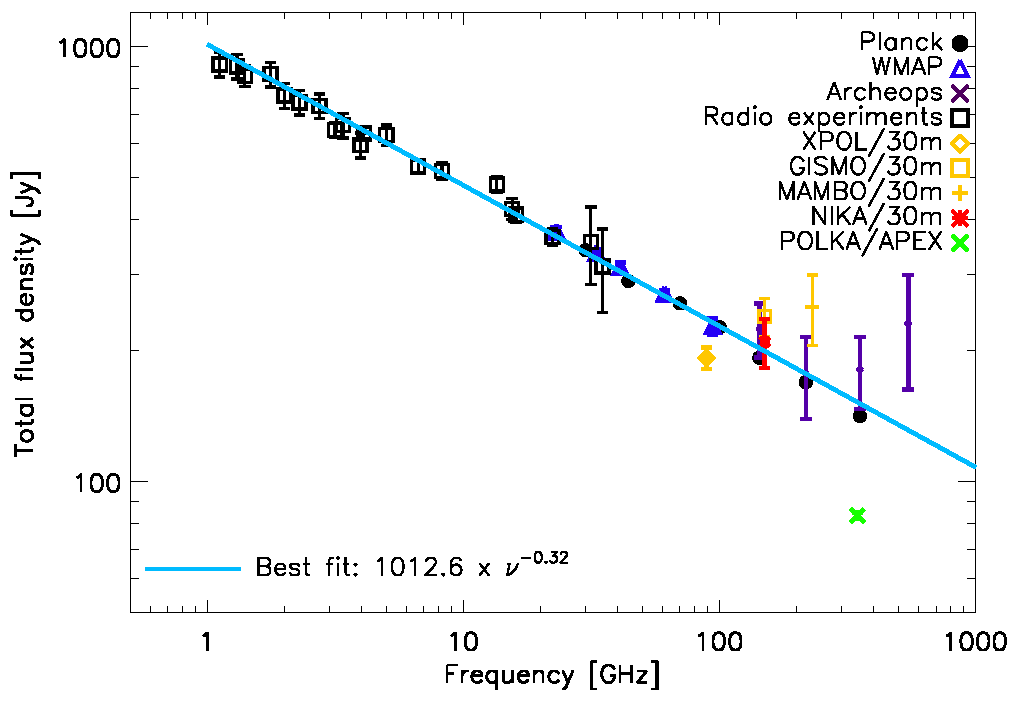
\includegraphics[width=1\linewidth,keepaspectratio]{figures/Crab_SED_int_test.pdf}}
           \caption{Crab nebula total power SED as obtained from \Planck\ \citep{2015arXiv150702058P}, \WMAP\ \citep{2011ApJS..192...19W}, Archeops \citep{macias2007archeops}, radio experiments \citep{dmitrenko1970absolute, 1971IzVUZ..14..157V}, XPOL/30m \citep{aumont2010}, \NIKA/30m (this paper), MAMBO/30m \citep{2002A&A...386.1044B}, POLKA/APEX \citep{2014PASP..126.1027W} and GISMO/30m \citep{2011ApJ...734...54A} data. \NIKA\ and POLKA values are estimated over the entire extend of the source. The best-fit single power law model obtained by the analysis in this paper is shown in cyan. Both, the best-fit models and the data account for the Crab nebula fading with time, using 2018 as year of reference. The POLKA data flux loss ($\sim$40\%) is compatible with the losses expected due to the spatial filtering of total intensity in LABOCA data reduction \citep{2011A&A...527A.145B}.}
\label{crab_SED}		
  \end{figure} 

\section{Characterization of the Crab Spectral Energy Distribution in intensity and polarization}\label{sec:Polarization intensity Spectral Energy Density (SED)}
\subsection{Intensity}
The total flux density of the Crab nebula at radio and millimeter
wavelengths (from 1 to 500 GHz) is mainly expected to be due to synchrotron emission and can be
well described by a single power law of the form:
\begin{equation}
I_{\nu} = A(\nu / 1 {\bf GHz})^{\beta}
\label{eq:sync1}
\end{equation}
with spectral index $\beta$ = -- 0.296$\pm$0.006 \citep{baars1977absolute,macias2010}. Further, the emission of the Crab nebula is fading with time at a rate of $\alpha$ = --0.167$\pm$0.015 \% yr$^{-1}$ \citep{aller1985decrease}. 
These results suggest a low frequency emission produced by particles accelerated by the same magnetic field. \cite{macias2010} have shown also that there is no evidence for an extra synchrotron component nor for thermal dust emission at these frequencies. The direction of the polarization is therefore expected to be constant across the frequency range 30-300 GHz while the polarization degree may vary.

Fig.~\ref{crab_SED} shows the total flux density of the Crab nebula as a function of the frequency. The fluxes in the radio domain were taken from \cite{dmitrenko1970absolute} and \cite{1971IzVUZ..14..157V}. We also show microwave and mm wavelengths fluxes from  \Archeops\ \citep{macias2007archeops}, \Planck\ \citep{2015arXiv150702058P}, \WMAP\ \citep{2011ApJS..192...19W}, XPOL/30m \citep{aumont2010}, MAMBO/30m \citep{2002A&A...386.1044B}, POLKA \citep{2014PASP..126.1027W} and GISMO/30m \citep{2011ApJ...734...54A}. The HFI \Planck\ data have been recomputed because of flux loss observed in previous results. These new results will be soon published by the \Planck\ collaboration. The measured \NIKA\ total flux density at 150 GHz is shown in red. 
Notice that in the plot both the best-fit model and the data represented are corrected for the fading of the source.

Assuming the single power law model in Eq.~\ref{eq:sync1} and
by $\chi^2$-minimization we obtain:
$$\setlength\arraycolsep{0.1em}
 \begin{array}{rclcl}
  \textrm{A}&=& 1012.6\pm3.8 & & \textrm{Jy}; \quad \quad  \textrm{$\beta$} = - 0.324\pm0.001\\
 \end{array}
$$
The best-fit model is shown in Fig.~\ref{crab_SED} in cyan.
The \NIKA\ data are consistent with this model at 1$\sigma$ level.
The estimated spectral index $\beta$ is slightly different from previous results provided by \cite{macias2010}. This 
is probably due to the addition of new \Planck\ and  WMAP data.

As already discussed above, XPOL total power emission is low with respect to expectations.
The POLKA value is found lower than \Planck\ result at the same frequency, this is mainly explained by the spatial filtering of LABOCA data reduction as already discussed in the previous section.
  
%\textbf{This section figures out a clear inconsistency of recent \Planck\ data with low and high frequency data. In particular they show the evidence of a break in the power law around 90-100 GHz suggesting a different origin of the emission and/or the presence of a second population of electrons. This should be investigate more with high angular resolution observations which will permit to probe the small and large angular scales.}

\subsection{Polarization}
Though the total power emission of the Crab nebula has been monitored over decades across a large range of frequencies, the amount of polarization data is still lacking.
Recent results provided by
\Planck\ \citep{2015arXiv150702058P}, \WMAP\ \citep{2011ApJS..192...19W},
XPOL \citep{aumont2010} and POLKA \citep{2014PASP..126.1027W}, together with \NIKA\ allow us to trace the spectral energy distribution of the polarized emission as shown in Fig.~\ref{crab_SED_ipol}.  
Notice that the uncertainty for the \NIKA\ value includes also absolute calibration errors.  
Assuming a single power law synchtron emission, see Eq.~\ref{eq:sync1}, for the polarization emission of the Crab nebula and using $\chi^2$ fitting procedure we find:
$$
\setlength\arraycolsep{0.1em}
 \begin{array}{rclcl}
  \textrm{A$_{pol}$}&=& 78.98\pm7.82 & & \textrm{Jy}; \quad \textrm{$\beta_{pol}$} = - 0.35\pm0.03\\
 \end{array}
 $$
We observe that \NIKA, XPOL and POLKA results are consistent with the best-fit model at the 1$\sigma$ level.
We have also estimated the spectral index of the Crab nebula polarization
emission at high frequency using the map obtained by SCUPOL \citep{scubapol} at 352 GHz (850
$\mu$m) and the \NIKA\ map. Considering only the region observed by SCUPOL ($\sim$1.5$^{\prime}$) we
obtain $\beta_{pol}^{\small NIKA/SCUPOL} = -0.33 \pm 0.01$.
This result is in good agreement with the best-fit model spectral index presented above.

The polarization spectral index is consistent with the total power one confirming the synchrotron radiation as the fundamental mechanism that drives the polarization emission of the Crab nebula.


\begin{figure}
  \centering
             { 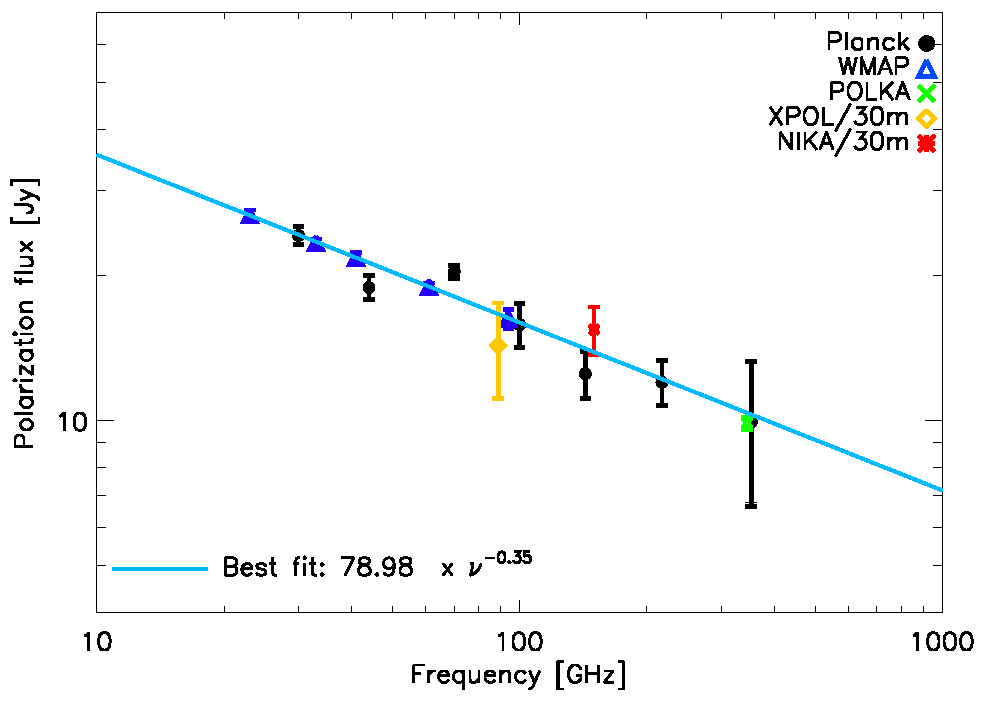
\includegraphics[width=1\linewidth,keepaspectratio]{figures/Crab_SED_ipol_test.pdf}}
           \caption{Crab nebula polarization flux SED as obtained from the \Planck\ \citep{2015arXiv150702058P}, \WMAP\ \citep{2011ApJS..192...19W}, XPOL \citep{aumont2010}, POLKA \citep{2014PASP..126.1027W} and \NIKA\ (this paper) data. \NIKA\ and POLKA values are estimated over the entire extend of the source. Both, the best-fit models and the data account for the Crab nebula fading with time, using 2018 as year of reference. We also show the single power law best-fit model in cyan.}
\label{crab_SED_ipol}		
  \end{figure} 
 \noindent



\section{Conclusions}\label{sec:conclusions}
The Crab nebula is considered as a celestial standard calibrator for CMB experiments in
terms of polarization degree and angle. An absolute calibration is
particularly important for reliable measurements of the CMB polarization B-modes,
which are a window towards the physics of the early Universe.

We have reported in this paper the first high angular resolution polarization observations of the Crab nebula at 150 GHz, obtained with the \NIKA\ camera. These observations have
allowed us to map the spatial distribution of the polarization
fraction and angle.  

Using the \NIKA\ data, in addition to the all available polarization data to date, we conclude that the
polarization angle of the Crab nebula is consistent with being constant with
frequency, from 20 GHz to 353 GHz, at arcmin scales with a value of
$-87.4^{\circ}\pm0.3$ in Galactic coordinates. High resolution observations provided by \NIKA\ at 150 GHz and POLKA at 345 GHz show
a polarization angle $\sim 3^{\circ}$ lower than the average value. Though the uncertainties on these values are high because of the systematic errors, this discrepancy highlights the need of further high angular resolution polarization observations in this frequency range.
In addition, we find a strong case for a constant polarization degree of $p$ = 6.95 $\pm$ 0.03\%. 

Moreover, we have characterized the intensity and polarization SED of the Crab nebula. In both total power and polarization, we find that the data are overall consistent with a single power law spectrum as expected from synchrotron emission from a single population of relativistic electrons.
We find that the Crab nebula presents a polarization spectral index which is consistent with the index in instensity. 
However, we find some discrepancies between data sets, which will require further mm measurements. Among future polarization experiments, \NIKAd\ \citep{calvo2016}, will provide high sensitive polarization observations of the Crab nebula adding a 260~GHz map at 11$^{\prime\prime}$ resolution.

\bibliography{bib_crab}

\vspace{0.2cm}
 \begin{acknowledgements}
We would like to thank the IRAM staff for their support during the \NIKA\ campaigns. 
The NIKA dilution cryostat has been designed and built at the Institut N\'eel. 
In particular, we acknowledge the crucial contribution of the Cryogenics Group, and 
in particular Gregory Garde, Henri Rodenas, Jean Paul Leggeri, Philippe Camus. 
This work has been partially funded by the Foundation Nanoscience Grenoble, the LabEx FOCUS ANR-11-LABX-0013 and 
the ANR under the contracts ``MKIDS'', ``NIKA'' and ANR-15-CE31-0017. 
This work has benefited from the support of the European Research Council Advanced Grant ORISTARS 
under the European Union's Seventh Framework Programme (Grant Agreement no. 291294).
We acknowledge fundings from the ENIGMASS French LabEx (R. A. and F. R.), 
the CNES post-doctoral fellowship program (R. A.), R.A. acknowledges support from Spanish Ministerio de Econom\'ia and Competitividad (MINECO) through grant number AYA2015-66211-C2-2, the CNES doctoral fellowship program (A. R.) and
the FOCUS French LabEx doctoral fellowship program (A. R.).
A.M. has received funding from the European Research Council (ERC) under the European Union’s Horizon 2020 research and innovation programme (MagneticYSOs, grant agreement No 679937).
\end{acknowledgements}





\end{document}
